\chapter{Additional graphs and spectra}

\newpage
\section{NICS of all sunflowers}
This sections includes the results for the NICS calculations described in \refsec{nics} applied to all of the isolated sunflower molecules.

All of the systems except for the As and P families have magnetic properties that hint towards aromaticity.
As08, P08 and P10 are clearly antiaromatic.
As10 has a less clear profile, but also seems to tend to antiaromaticy.
As12 and P12 are the less clear of them all, but also seem to have an antiaromatic magnetic behavior.

\begin{figure*}[h]
\centering
\begin{subfigure}{5.5cm}\centering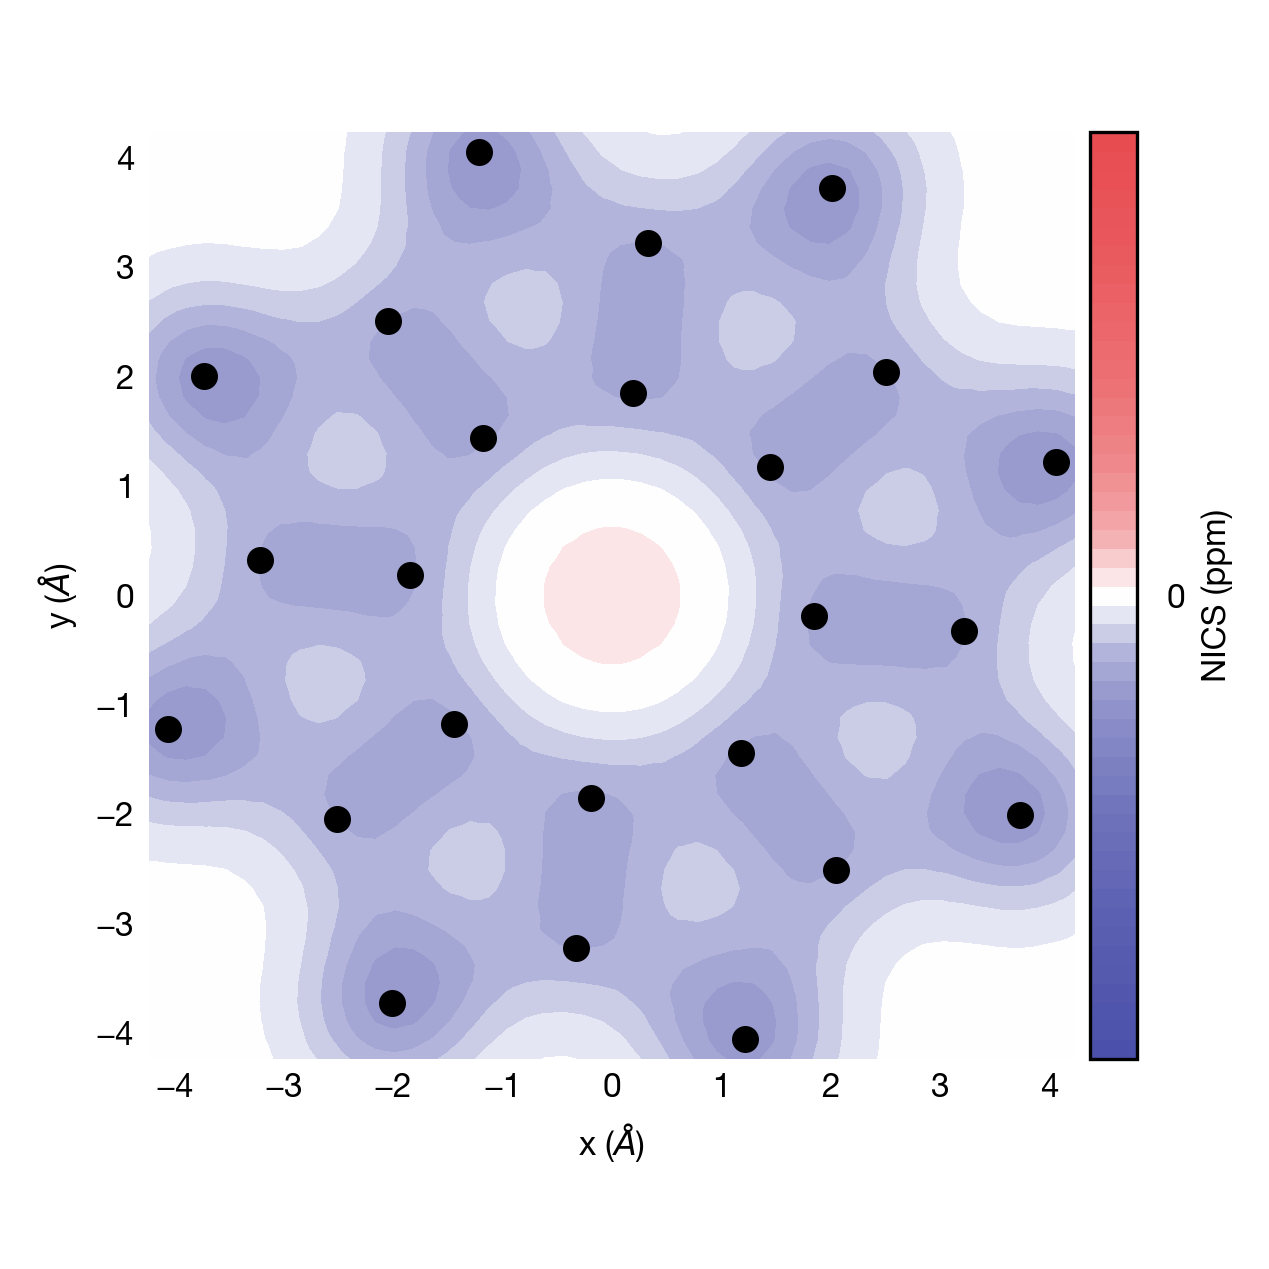
\includegraphics{s08-2d}\caption{NICS 2D projection for S08.\\Aromatic character}\end{subfigure}%
\begin{subfigure}{5.5cm}\centering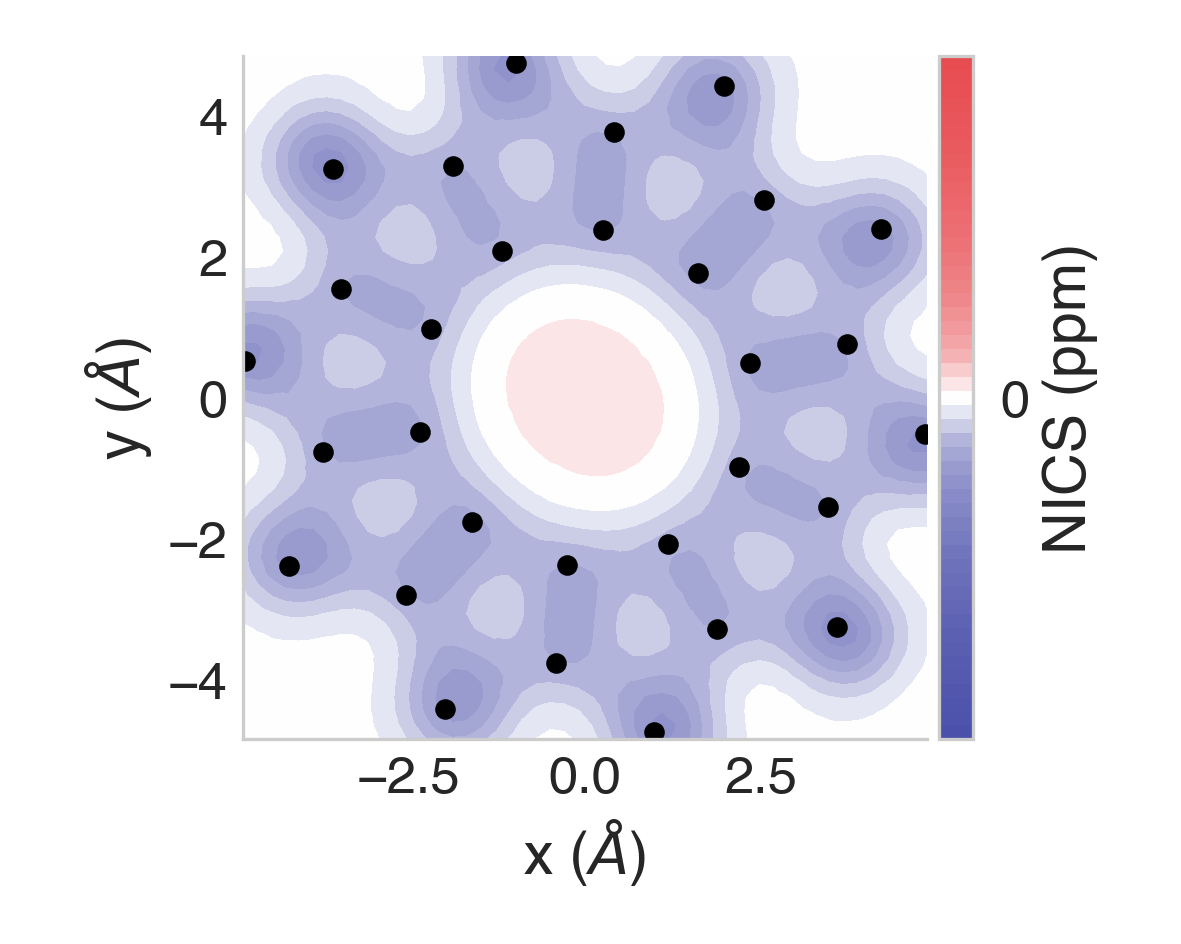
\includegraphics{s10-2d}\caption{NICS 2D projection for S10.\\Aromatic character}\end{subfigure}%
\begin{subfigure}{5.5cm}\centering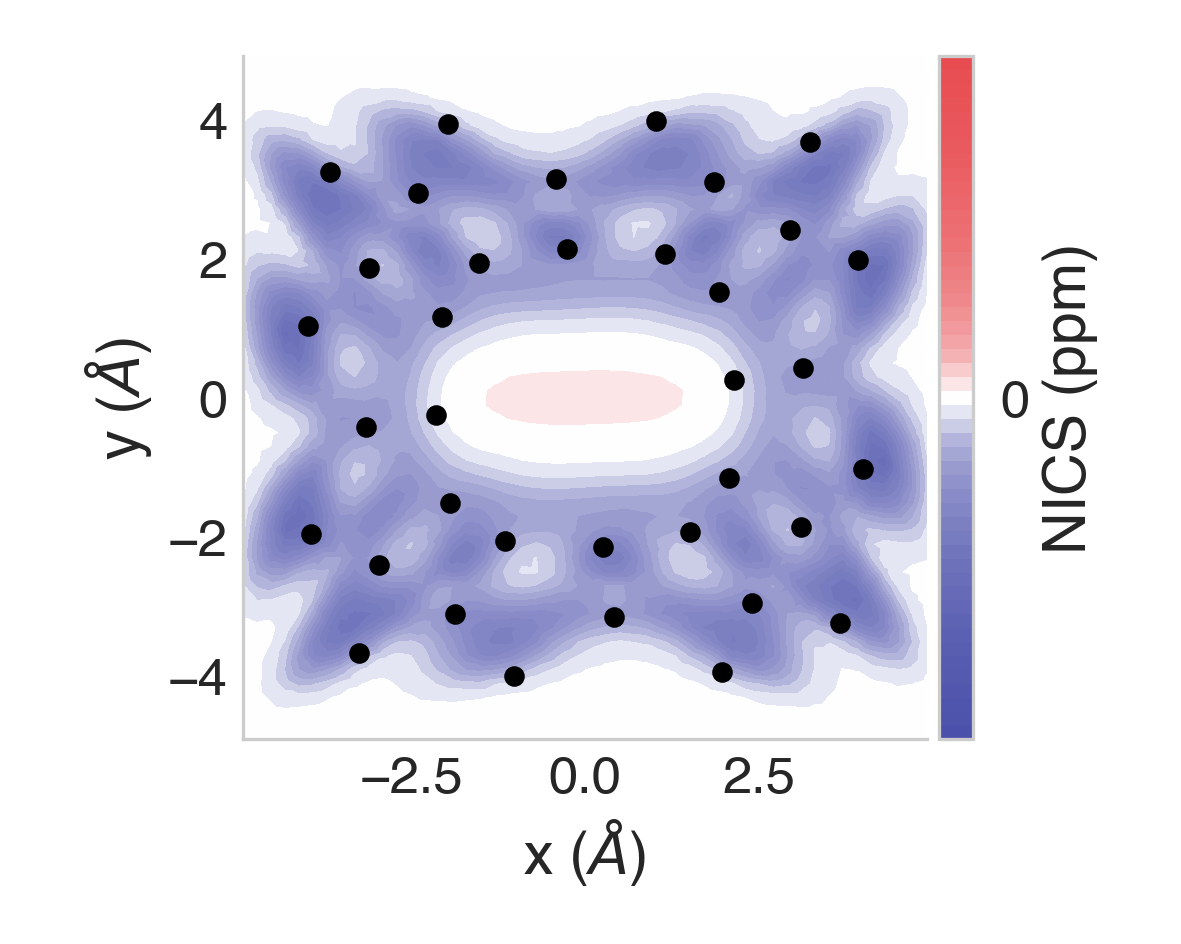
\includegraphics{s12-2d}\caption{NICS 2D projection for S12.\\Aromatic character}\end{subfigure}
\begin{subfigure}{5.5cm}\centering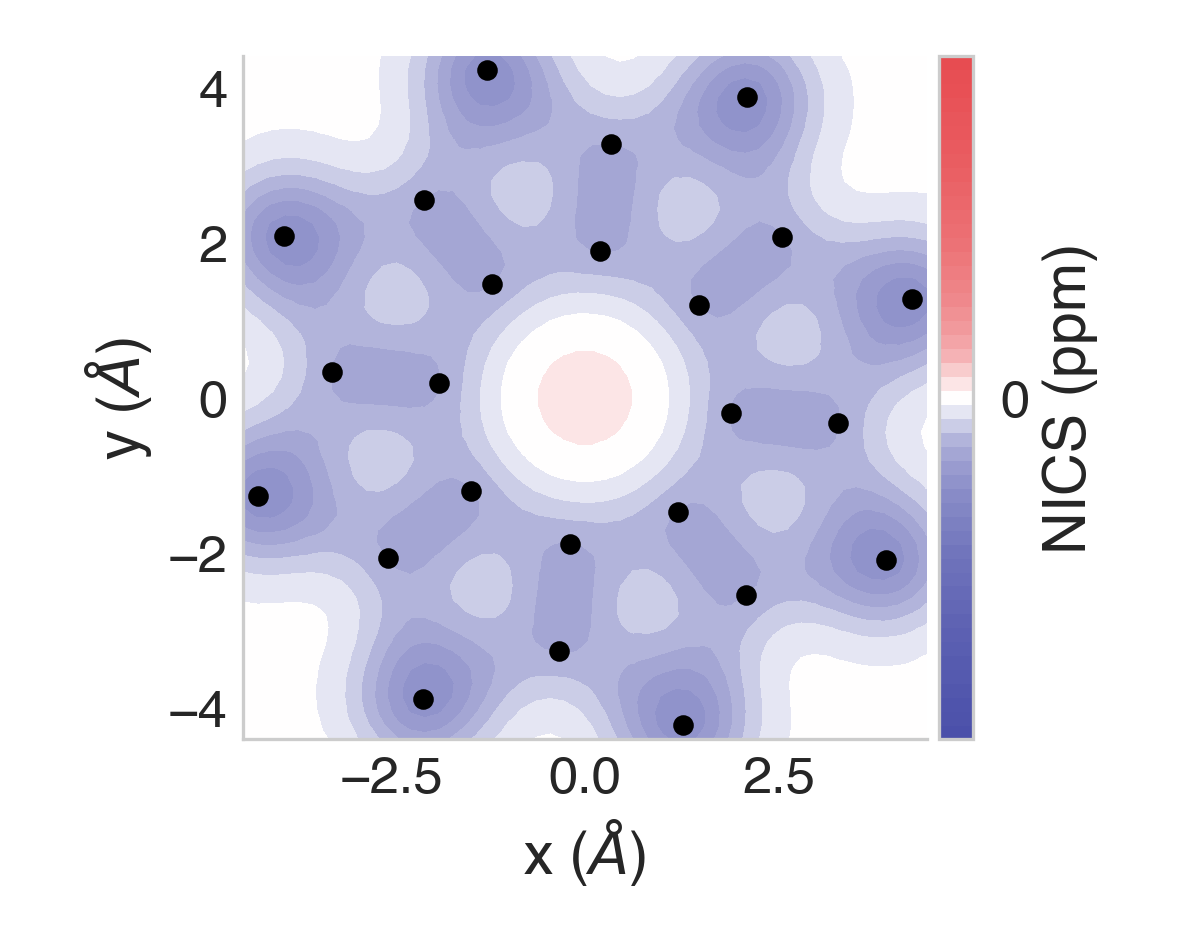
\includegraphics{se08-2d}\caption{NICS 2D projection for Se08.\\Aromatic character}\end{subfigure}%
\begin{subfigure}{5.5cm}\centering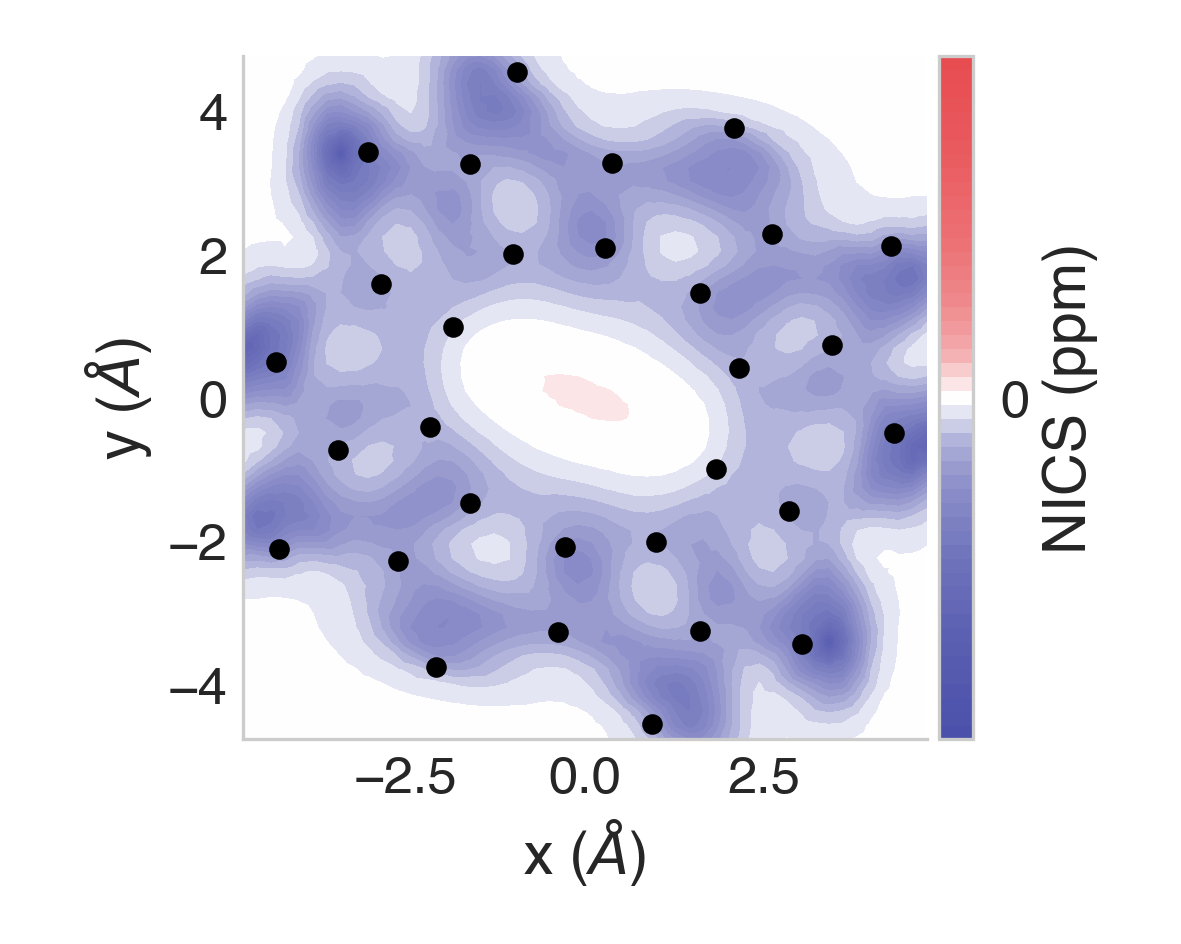
\includegraphics{se10-2d}\caption{NICS 2D projection for Se10.\\Aromatic character}\end{subfigure}%
\begin{subfigure}{5.5cm}\centering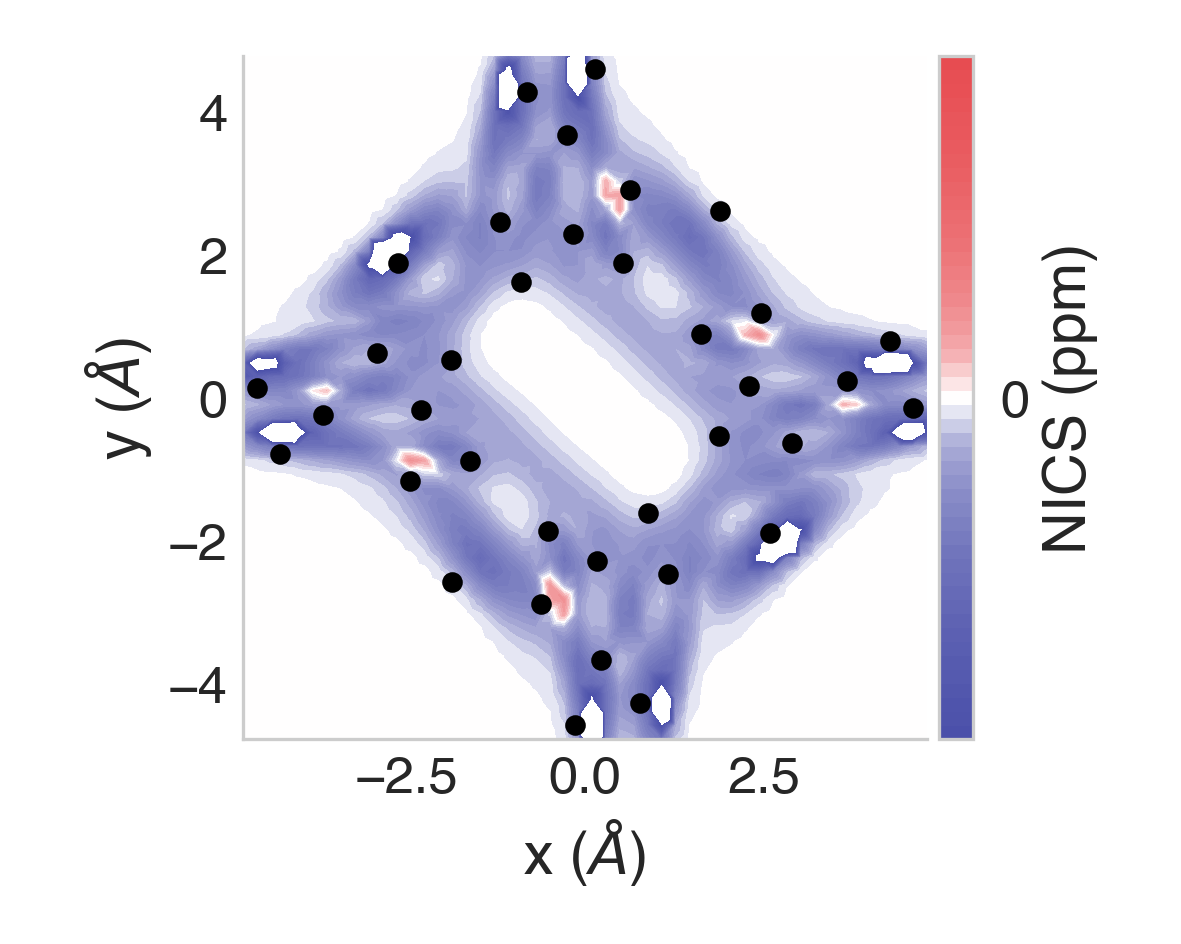
\includegraphics{se12-2d}\caption{NICS 2D projection for Se12.\\Aromatic character}\end{subfigure}
\begin{subfigure}{5.5cm}\centering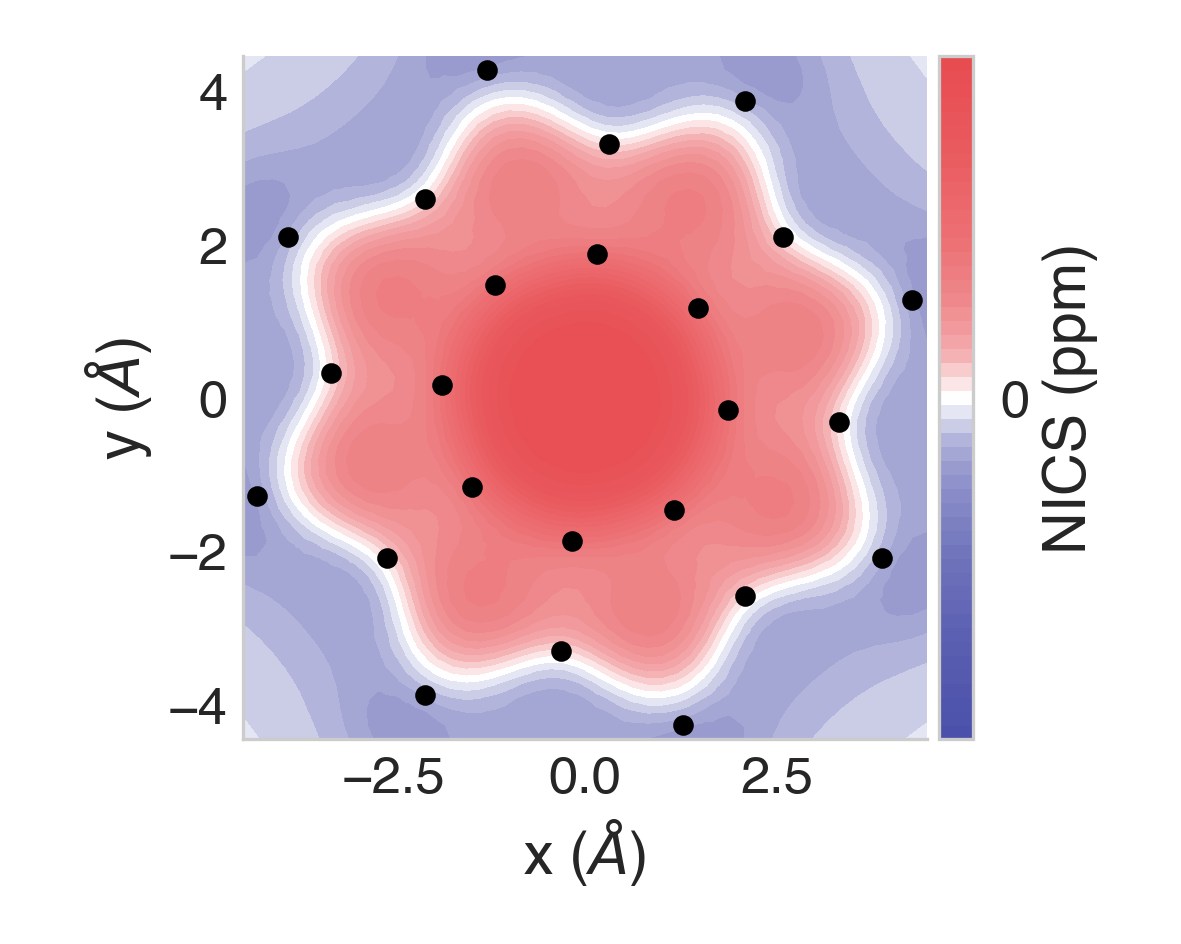
\includegraphics{as08-2d}\caption{NICS 2D projection for As08.\\Antiaromatic character}\end{subfigure}%
\begin{subfigure}{5.5cm}\centering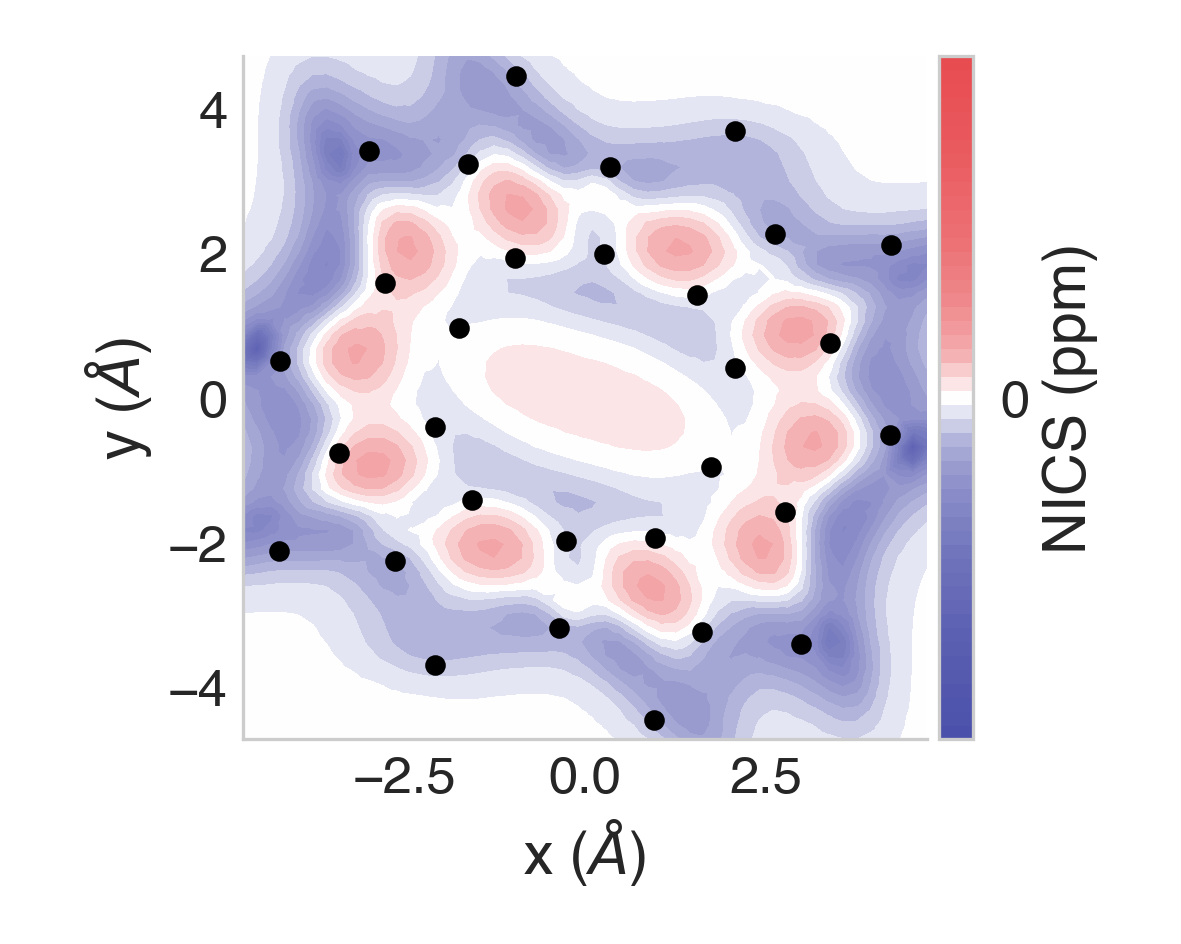
\includegraphics{as10-2d}\caption{NICS 2D projection for As10.\\Unclear but hints antiaromaticity}\end{subfigure}%
\begin{subfigure}{5.5cm}\centering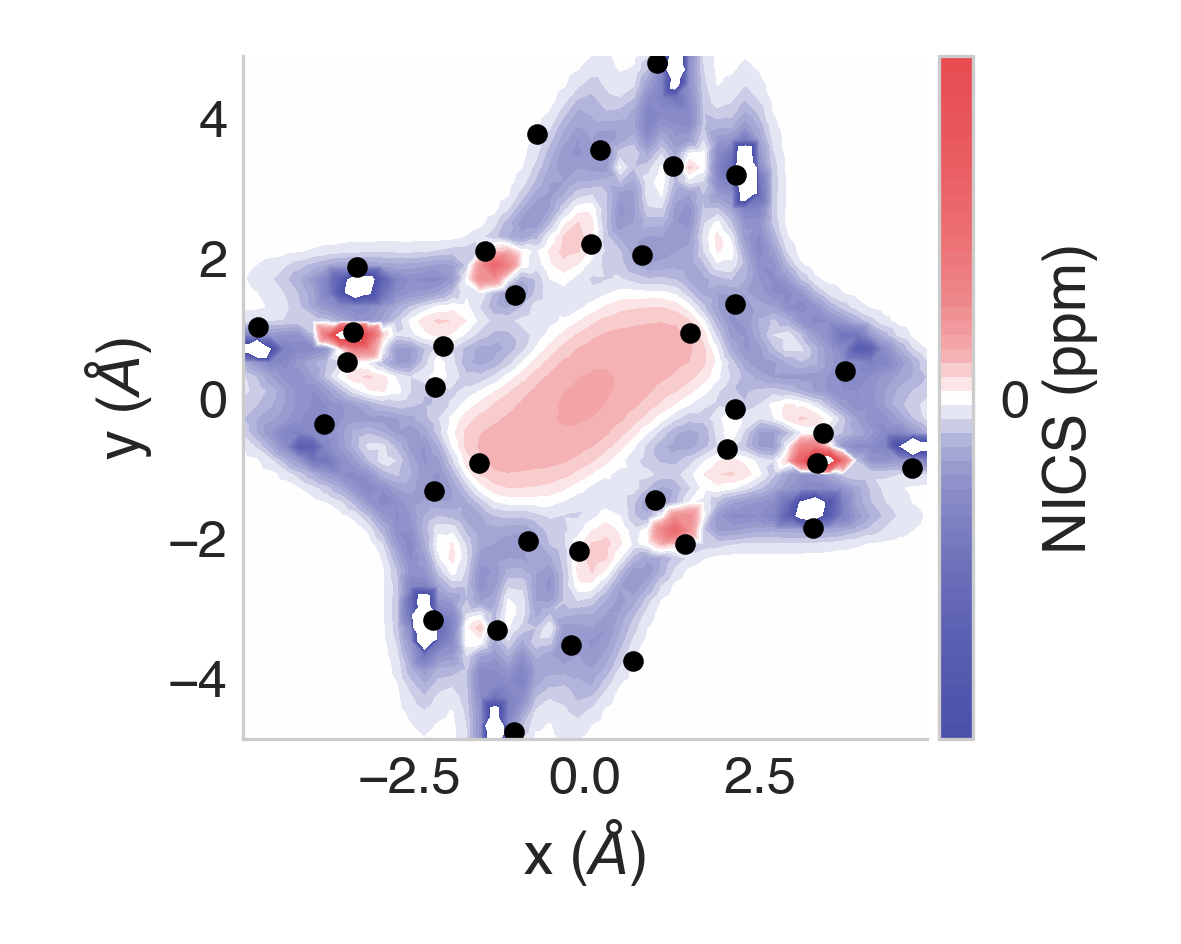
\includegraphics{as12-2d}\caption{NICS 2D projection for As12.\\Unclear tendency, possibly antiaromatic}\end{subfigure}
\caption[Part 1 of NICS 2D projections]{Part 1 of NICS 2D projections}
\end{figure*}

\newpage

\begin{figure*}[h]
\centering
\begin{subfigure}{5.5cm}\centering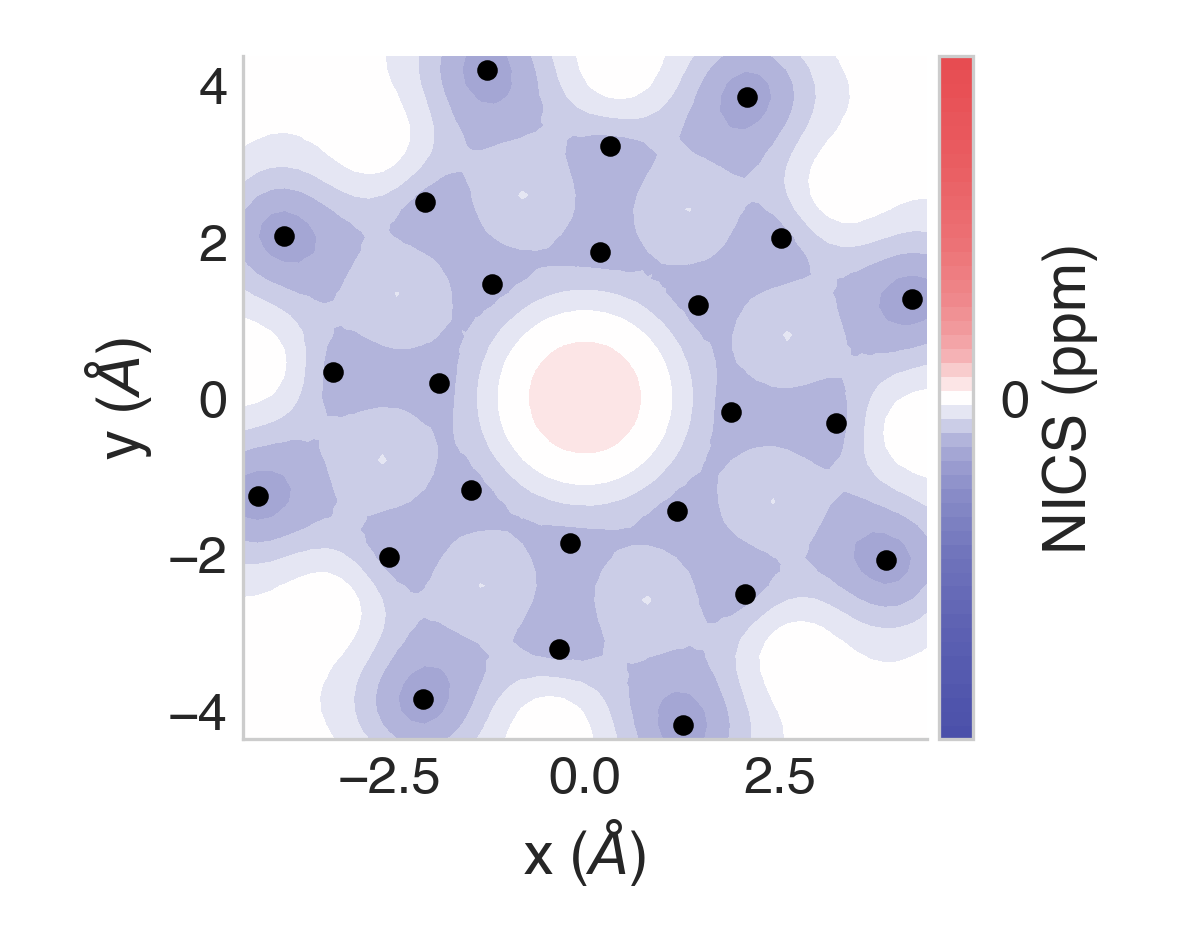
\includegraphics{asn08-2d}\caption{NICS 2D projection for AsN08.\\Aromatic character}\end{subfigure}%
\begin{subfigure}{5.5cm}\centering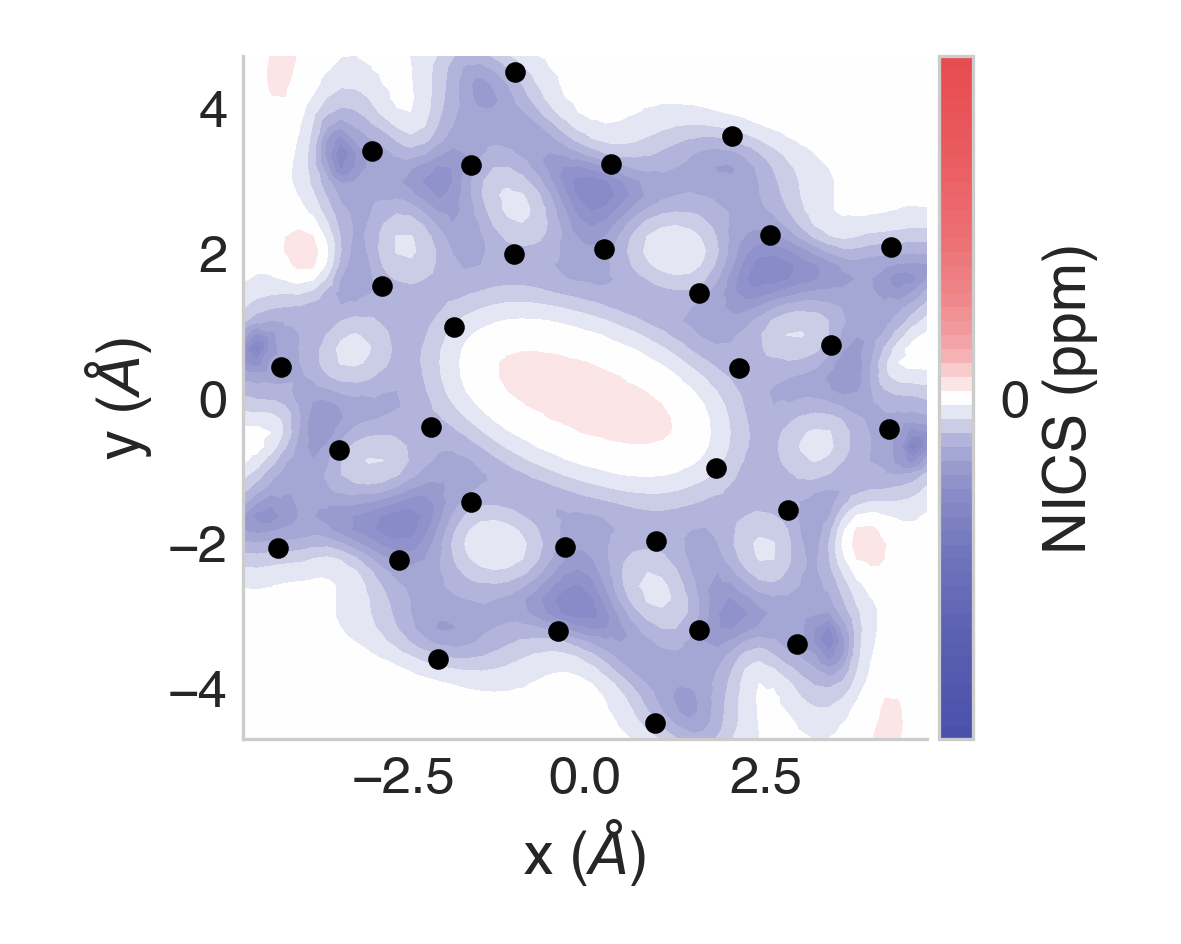
\includegraphics{asn10-2d}\caption{NICS 2D projection for AsN10.\\Aromatic character}\end{subfigure}%
\begin{subfigure}{5.5cm}\centering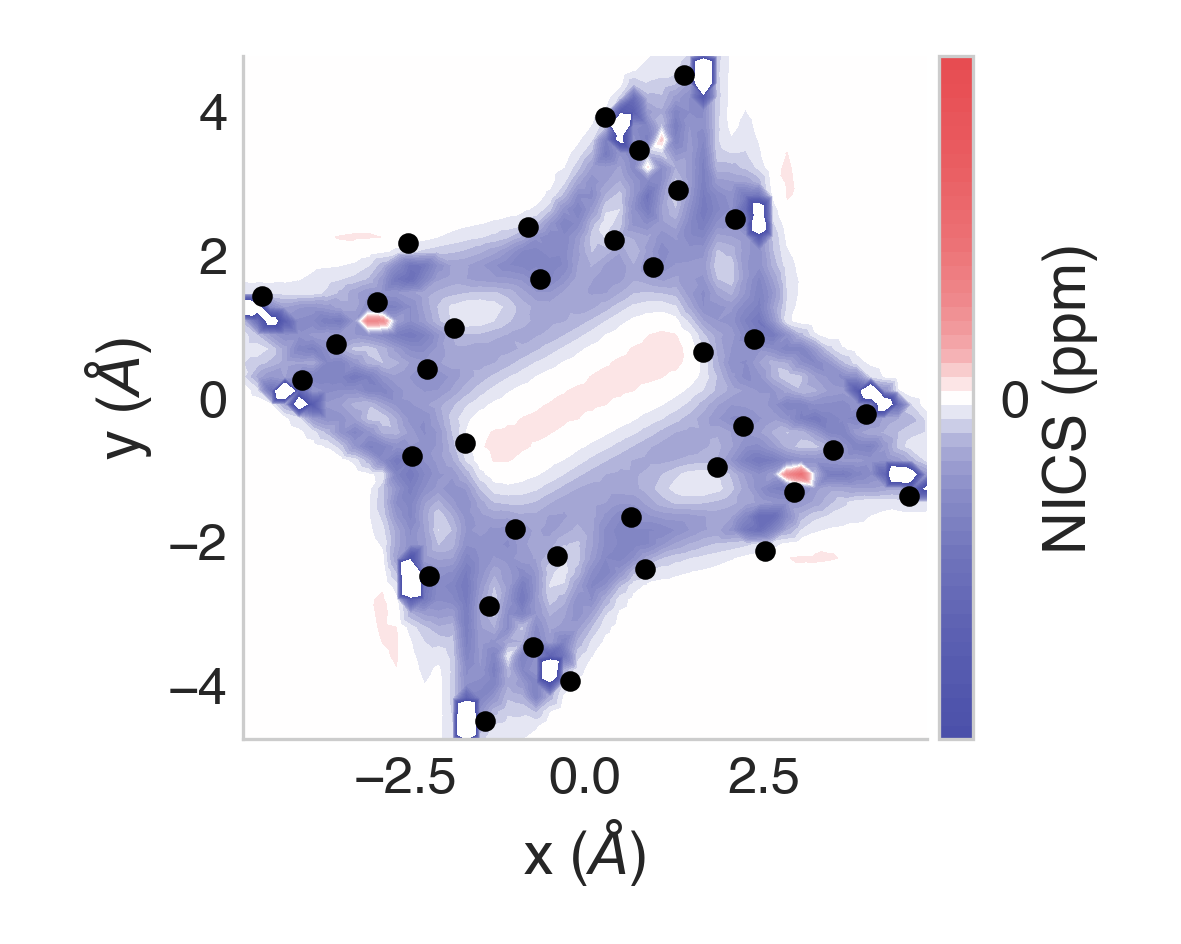
\includegraphics{asn12-2d}\caption{NICS 2D projection for AsN12.\\Aromatic character}\end{subfigure}
\begin{subfigure}{5.5cm}\centering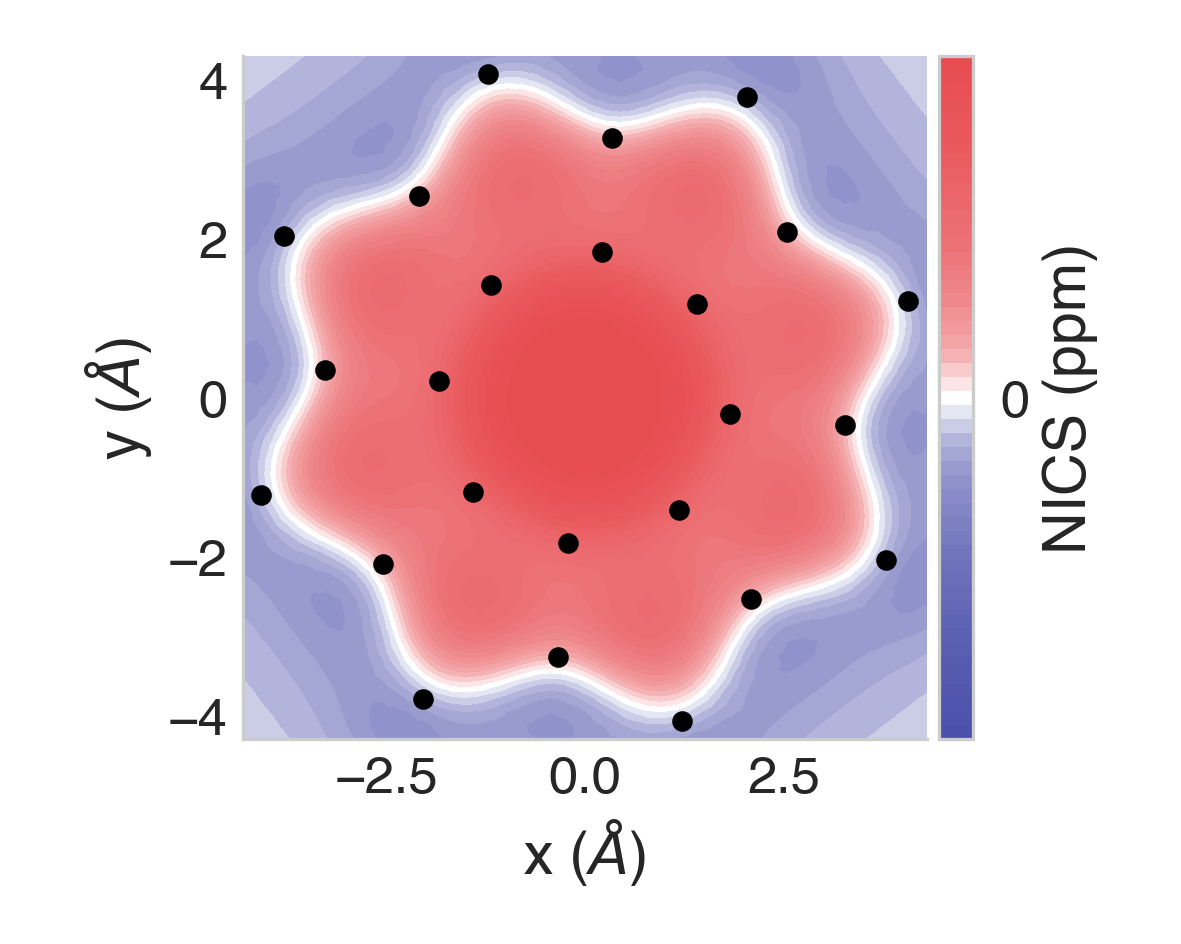
\includegraphics{p08-2d}\caption{NICS 2D projection for P08.\\Antiaromatic character}\end{subfigure}%
\begin{subfigure}{5.5cm}\centering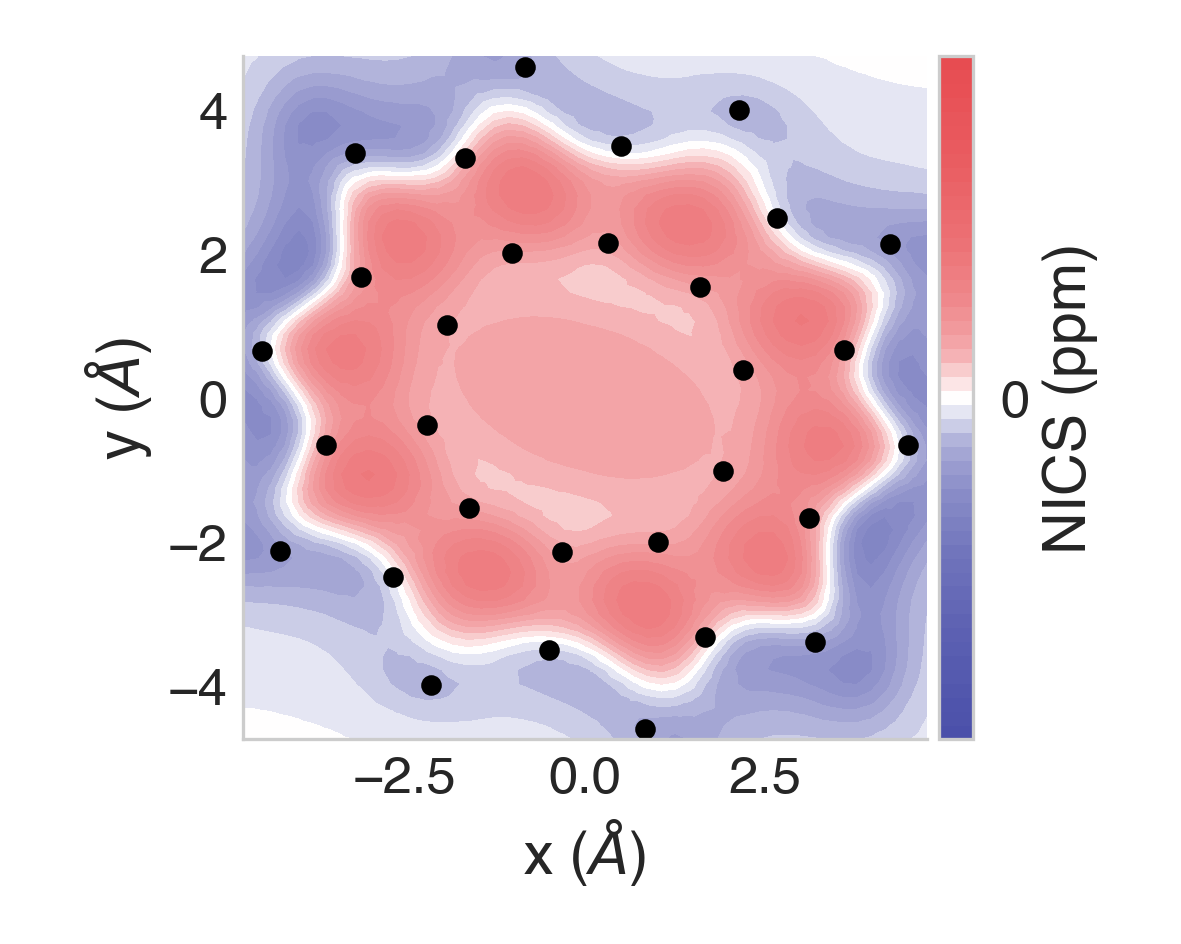
\includegraphics{p10-2d}\caption{NICS 2D projection for P10.\\Antiaromatic character}\end{subfigure}%
\begin{subfigure}{5.5cm}\centering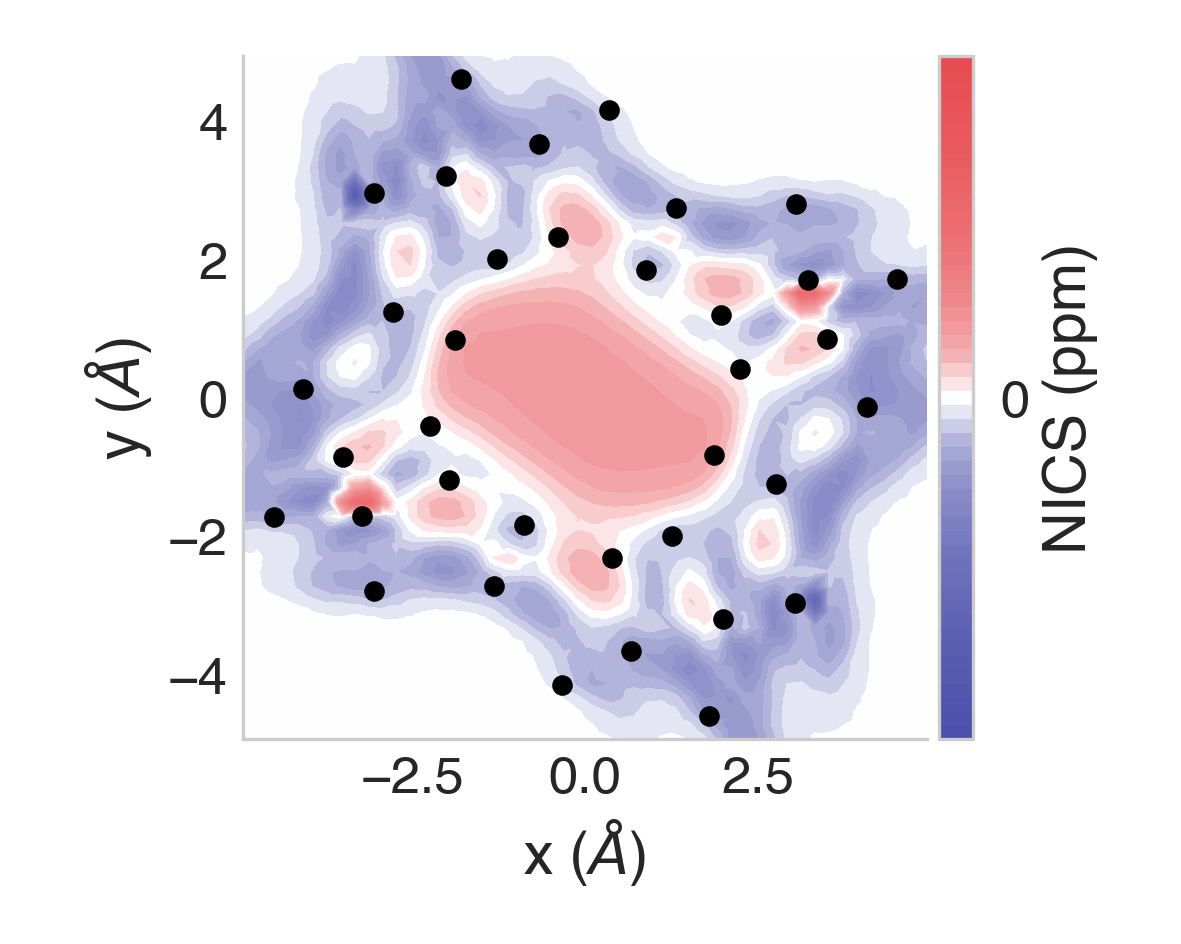
\includegraphics{p12-2d}\caption{NICS 2D projection for P12.\\Unclear tendency, possibly antiaromatic}\end{subfigure}
\begin{subfigure}{5.5cm}\centering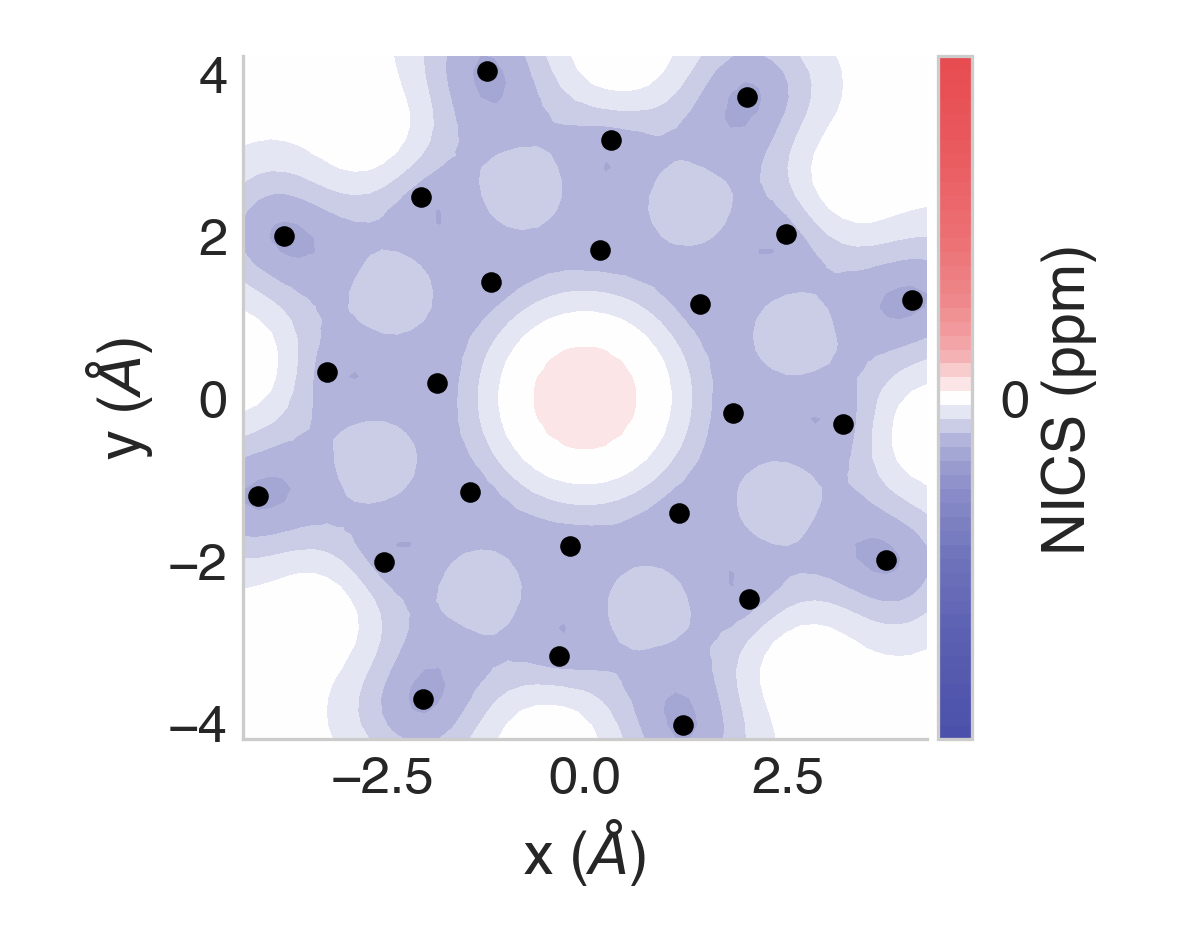
\includegraphics{pn08-2d}\caption{NICS 2D projection for PN08.\\Aromatic character}\end{subfigure}%
\begin{subfigure}{5.5cm}\centering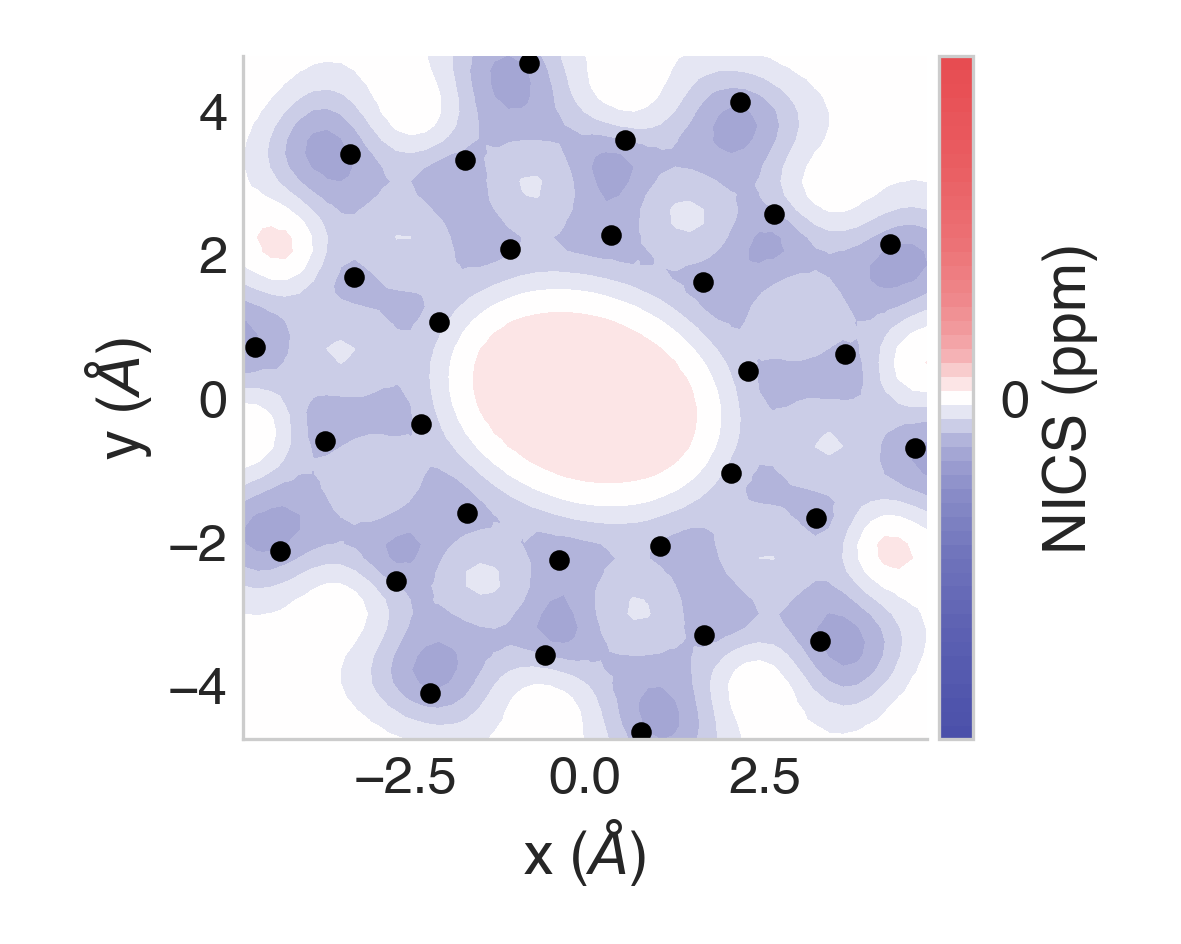
\includegraphics{pn10-2d}\caption{NICS 2D projection for PN10.\\Aromatic character}\end{subfigure}%
\begin{subfigure}{5.5cm}\centering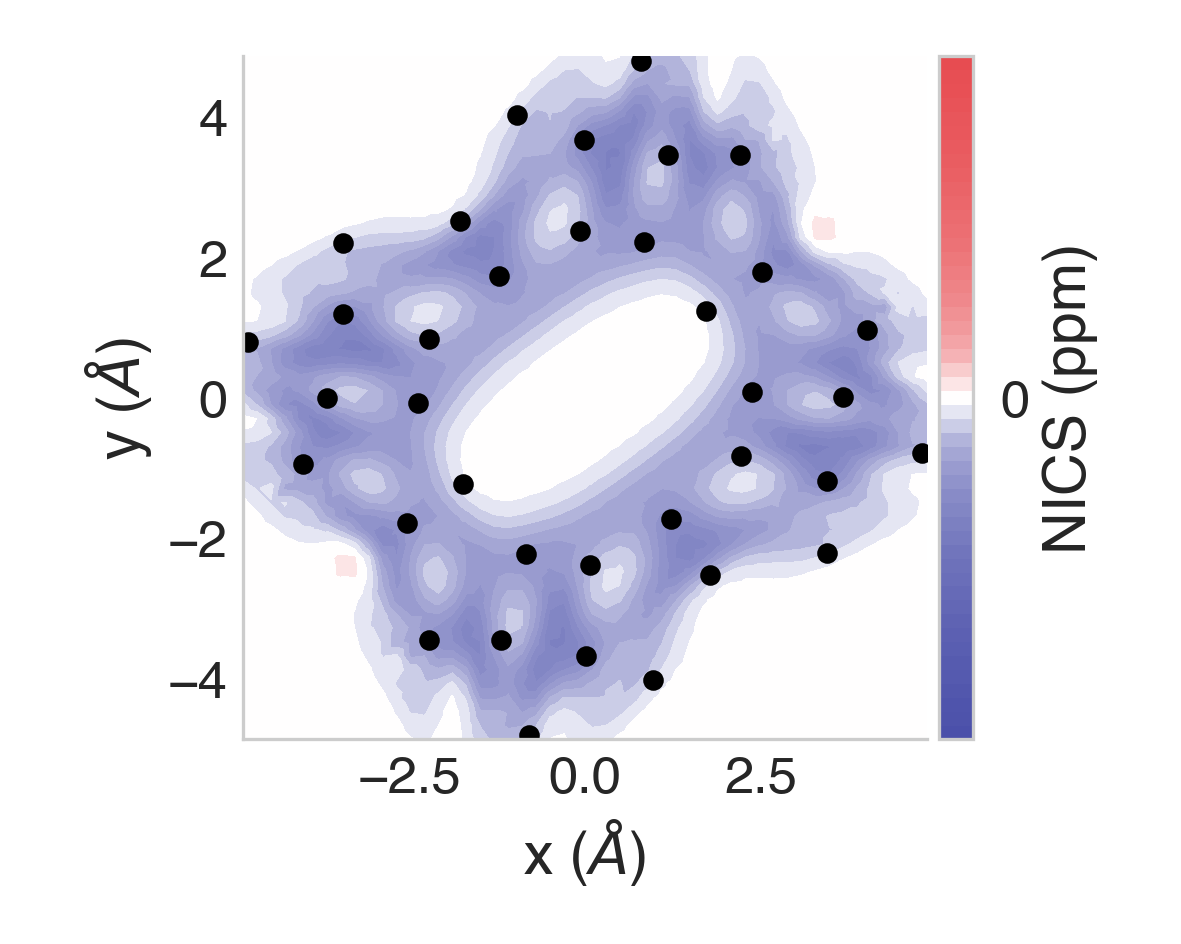
\includegraphics{pn12-2d}\caption{NICS 2D projection for PN12.\\Aromatic character}\end{subfigure}
\caption[Part 2 of NICS 2D projections]{Part 2 of NICS 2D projections}
\end{figure*}


\newpage
\section{Raman spectra of all sunflowers}


\newpage
\section{UV-vis spectra of all sunflowers}
\labsec{ap:uv-vis-flowers}

As described in \refsec{uv-sunflowers}, \refsec{uv-stx} and \refsec{complex-uv}, UV-vis spectra was calculated and plotted for the lone sunflowers, the lone STX, and each of the flower-STX complexes.
The spectrum of each flower and spectrum the complex that it forms with STX have been displayed in the same graph for convenience and to allow for direct comparison.
The spectrum of lone STX has also been added as a reference.

\begin{figure*}[h]
\centering
\begin{subfigure}{8.25cm}\centering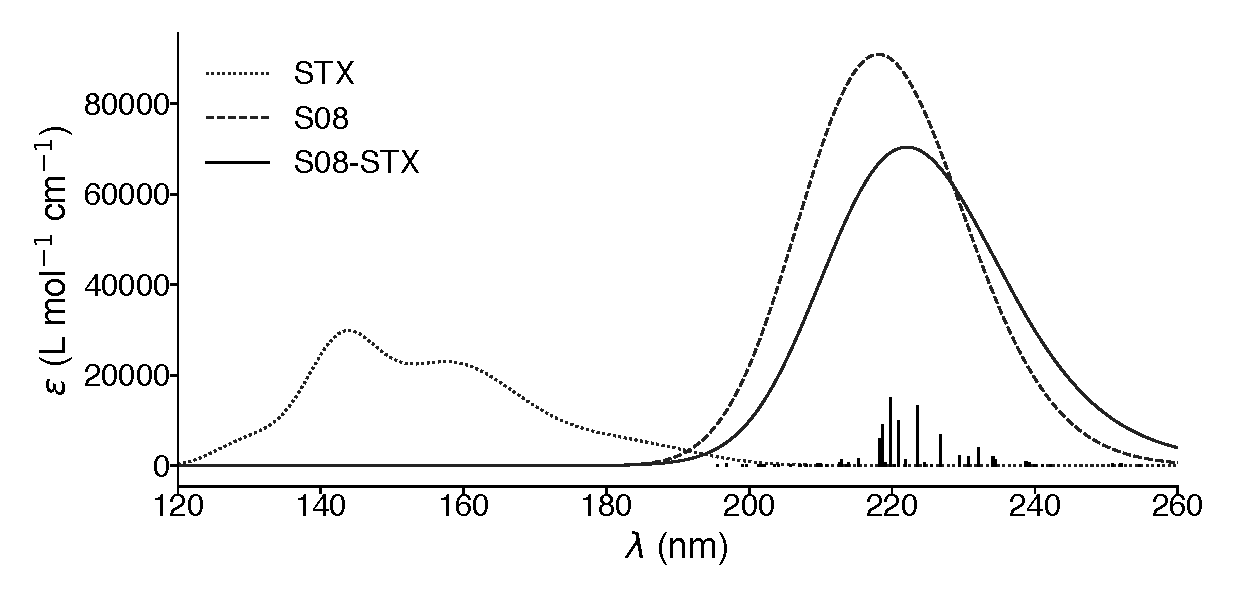
\includegraphics{uv-s08}\caption{UV-vis spectrum for S08}\end{subfigure}%
\begin{subfigure}{8.25cm}\centering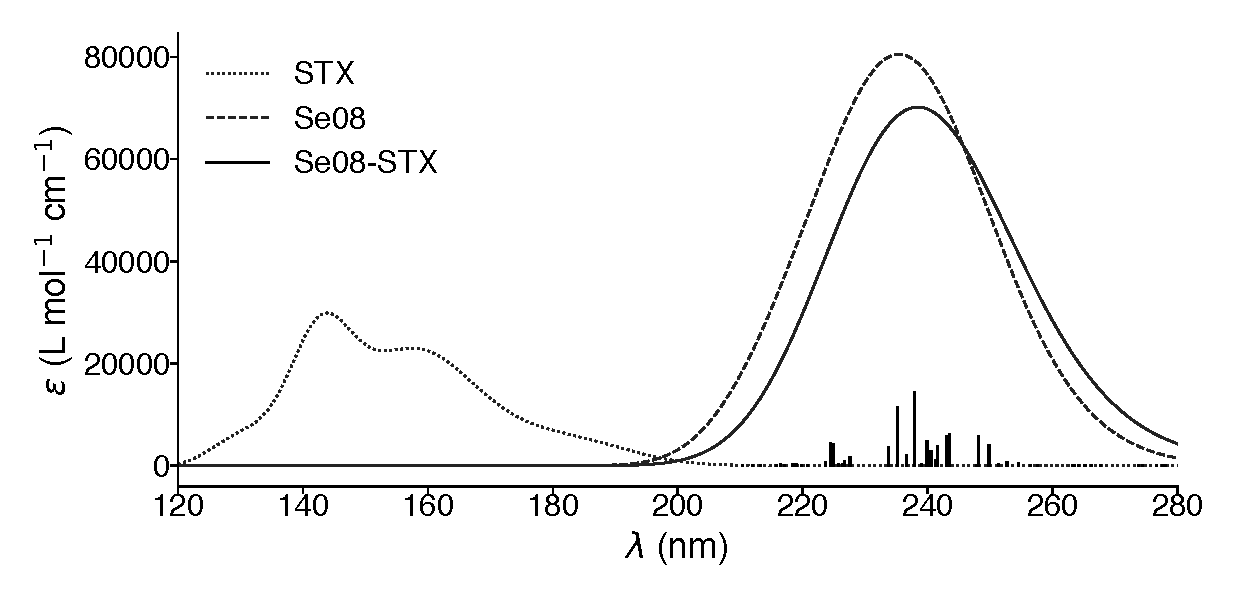
\includegraphics{uv-se08}\caption{UV-vis spectrum for Se08}\end{subfigure}
\begin{subfigure}{8.25cm}\centering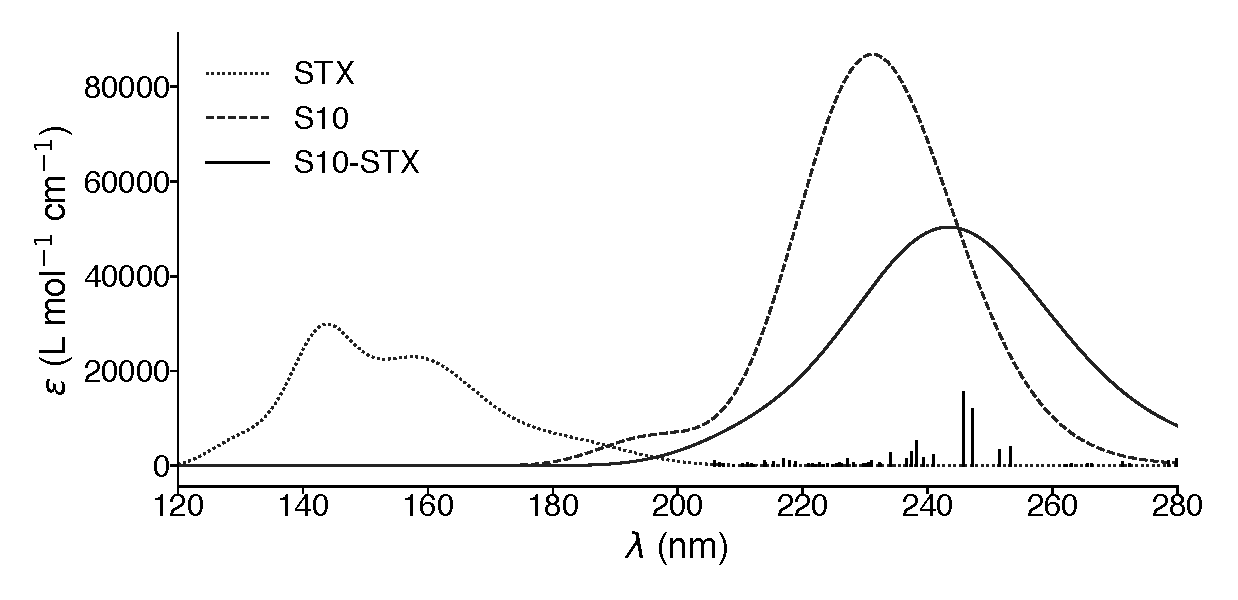
\includegraphics{uv-s10}\caption{UV-vis spectrum for S10}\end{subfigure}%
\begin{subfigure}{8.25cm}\centering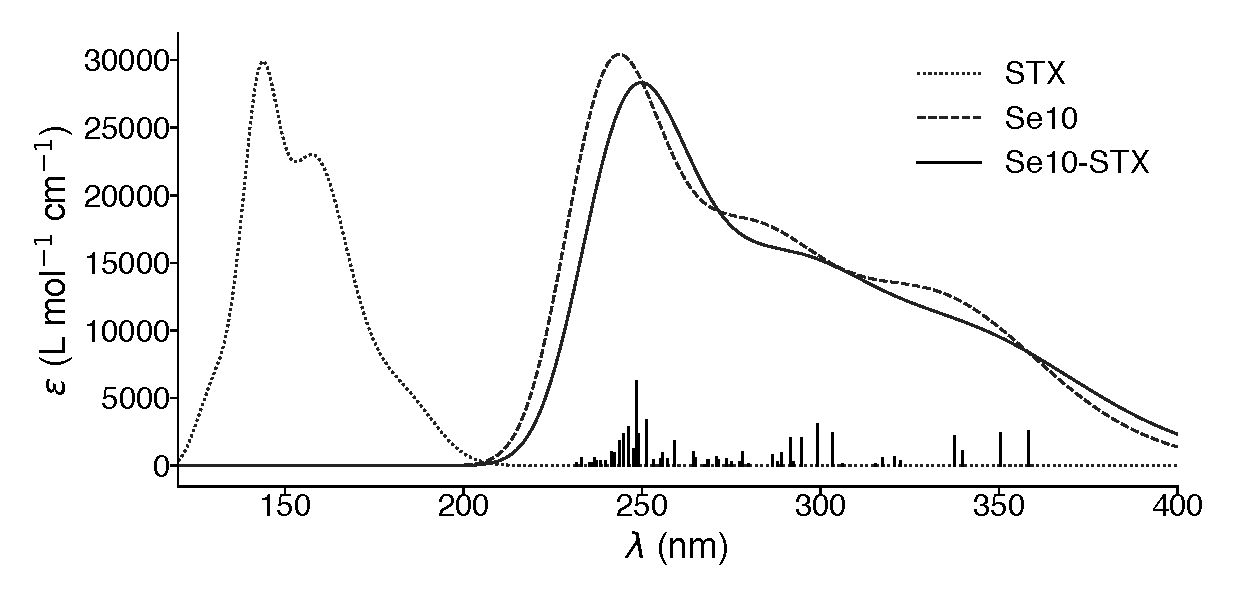
\includegraphics{uv-se10}\caption{UV-vis spectrum for Se10}\end{subfigure}
\begin{subfigure}{8.25cm}\centering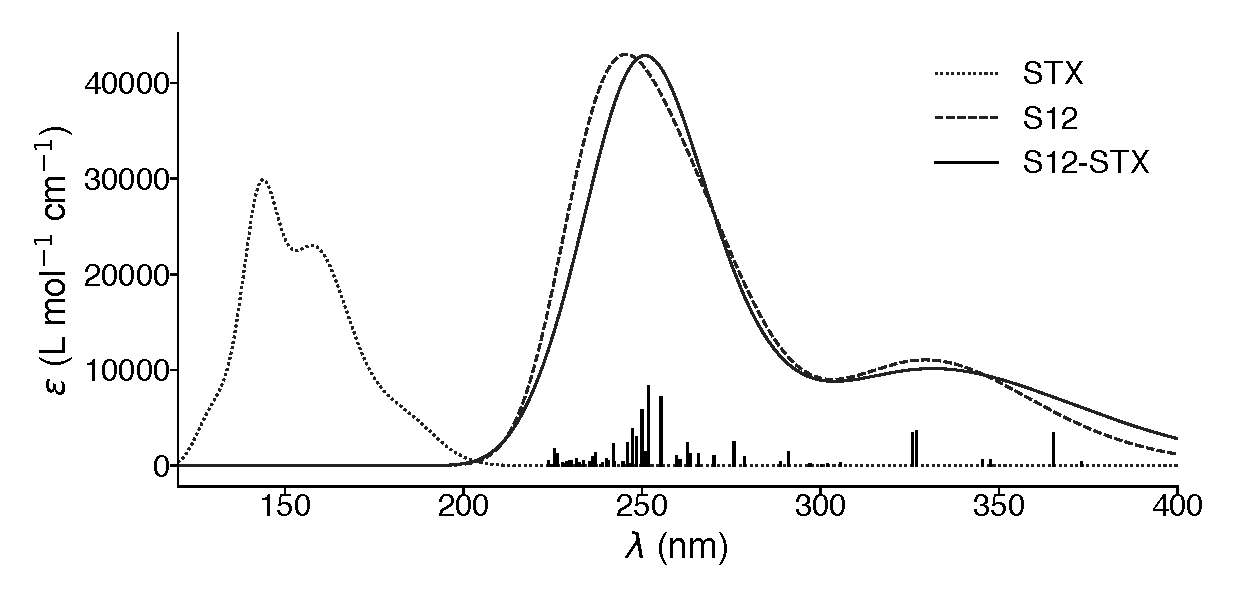
\includegraphics{uv-s12}\caption{UV-vis spectrum for S12}\end{subfigure}%
\begin{subfigure}{8.25cm}\centering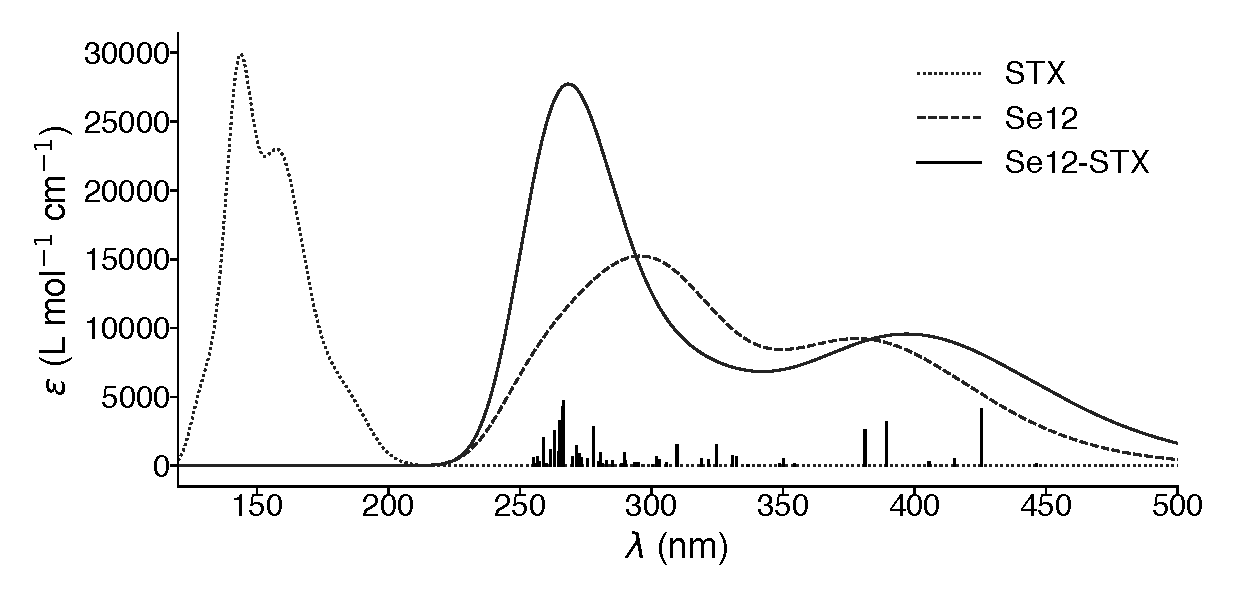
\includegraphics{uv-se12}\caption{UV-vis spectrum for Se12}\end{subfigure}
\caption[Part 1 of flower UV-vis spectra]{Part 1 of flower UV-vis spectra}
\end{figure*}

\newpage

\begin{figure*}[h]
\centering
\begin{subfigure}{8.25cm}\centering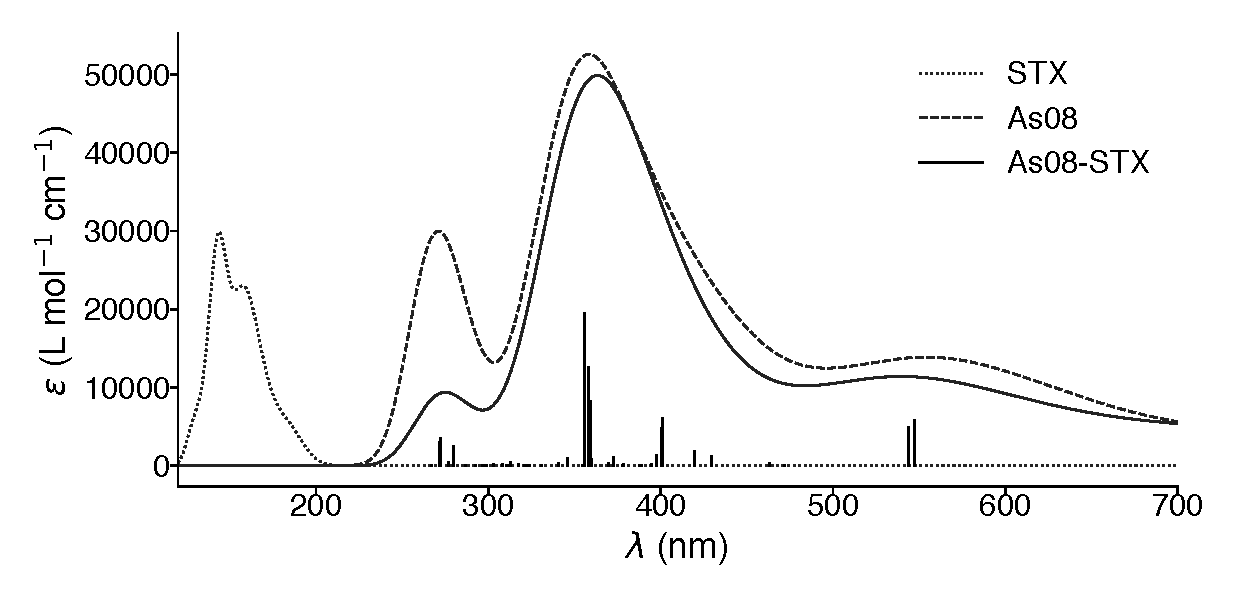
\includegraphics{uv-as08}\caption{UV-vis spectrum for As08}\end{subfigure}%
\begin{subfigure}{8.25cm}\centering\includegraphics{uv-asn08}\caption{UV-vis spectrum for AsN08}\end{subfigure}
\begin{subfigure}{8.25cm}\centering\includegraphics{uv-as10}\caption{UV-vis spectrum for As10}\end{subfigure}%
\begin{subfigure}{8.25cm}\centering\includegraphics{uv-asn10}\caption{UV-vis spectrum for AsN10}\end{subfigure}
\begin{subfigure}{8.25cm}\centering\includegraphics{uv-as12}\caption{UV-vis spectrum for As12}\end{subfigure}%
\begin{subfigure}{8.25cm}\centering\includegraphics{uv-asn12}\caption{UV-vis spectrum for AsN12}\end{subfigure}
\caption[Part 2 of flower UV-vis spectra]{Part 2 of flower UV-vis spectra}
\end{figure*}

\newpage

\begin{figure*}[h]
\centering
\begin{subfigure}{8.25cm}\centering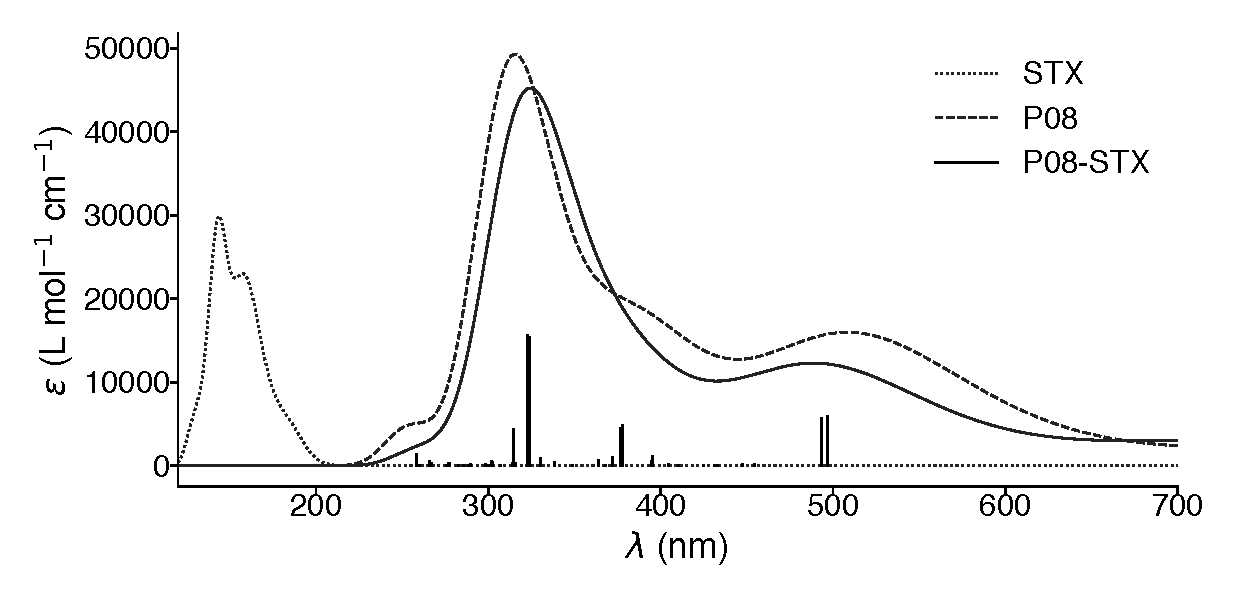
\includegraphics{uv-p08}\caption{UV-vis spectrum for P08}\end{subfigure}%
\begin{subfigure}{8.25cm}\centering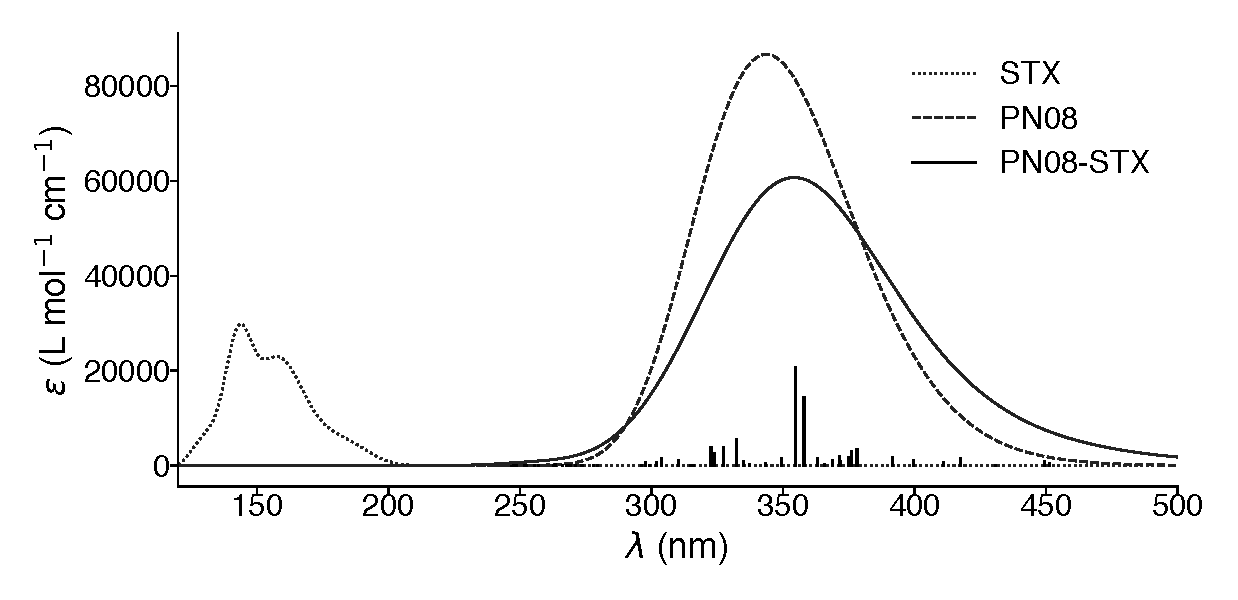
\includegraphics{uv-pn08}\caption{UV-vis spectrum for PN08}\end{subfigure}
\begin{subfigure}{8.25cm}\centering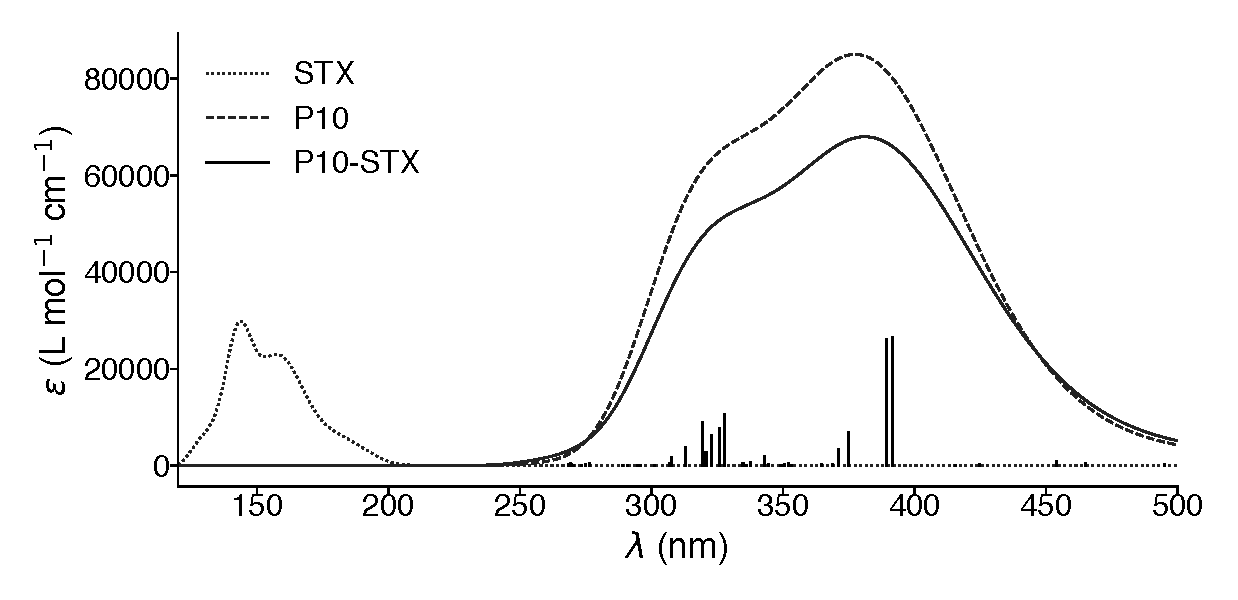
\includegraphics{uv-p10}\caption{UV-vis spectrum for P10}\end{subfigure}%
\begin{subfigure}{8.25cm}\centering\includegraphics{uv-pn10}\caption{UV-vis spectrum for PN10}\end{subfigure}
\begin{subfigure}{8.25cm}\centering\includegraphics{uv-p12}\caption{UV-vis spectrum for P12}\end{subfigure}%
\begin{subfigure}{8.25cm}\centering\includegraphics{uv-pn12}\caption{UV-vis spectrum for PN12}\end{subfigure}
\caption[Part 3 of flower UV-vis spectra]{Part 3 of flower UV-vis spectra}
\end{figure*}


\newpage
\section{Combined enhancement factor graphs}
\labsec{ap:combined-ef}

\begin{figure*}[h]
\centering
\begin{subfigure}{8.25cm}\centering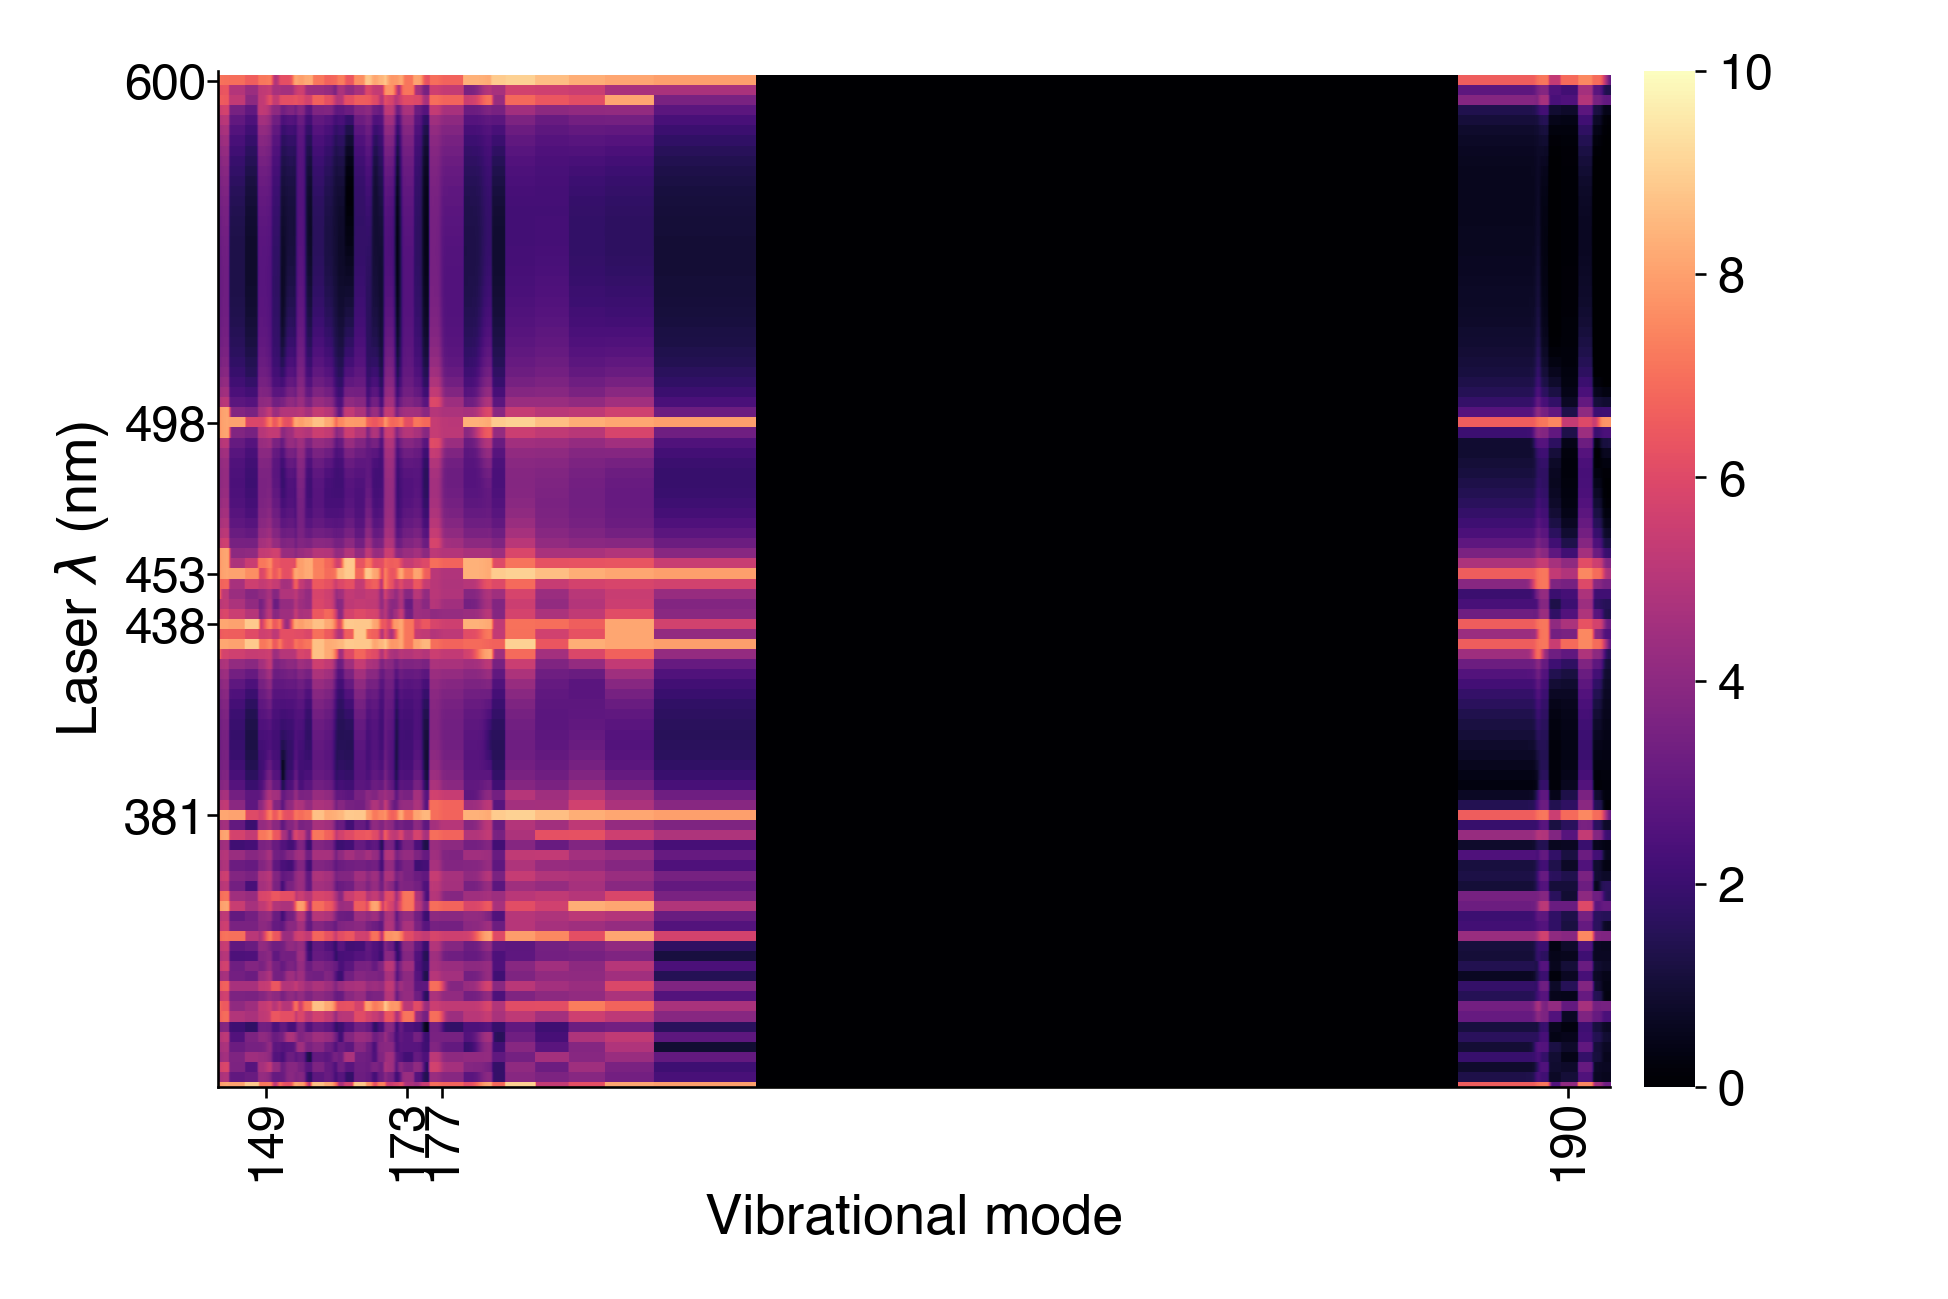
\includegraphics{comb-as10}\caption{Combined graph for As10-STX}\end{subfigure}%
\begin{subfigure}{8.25cm}\centering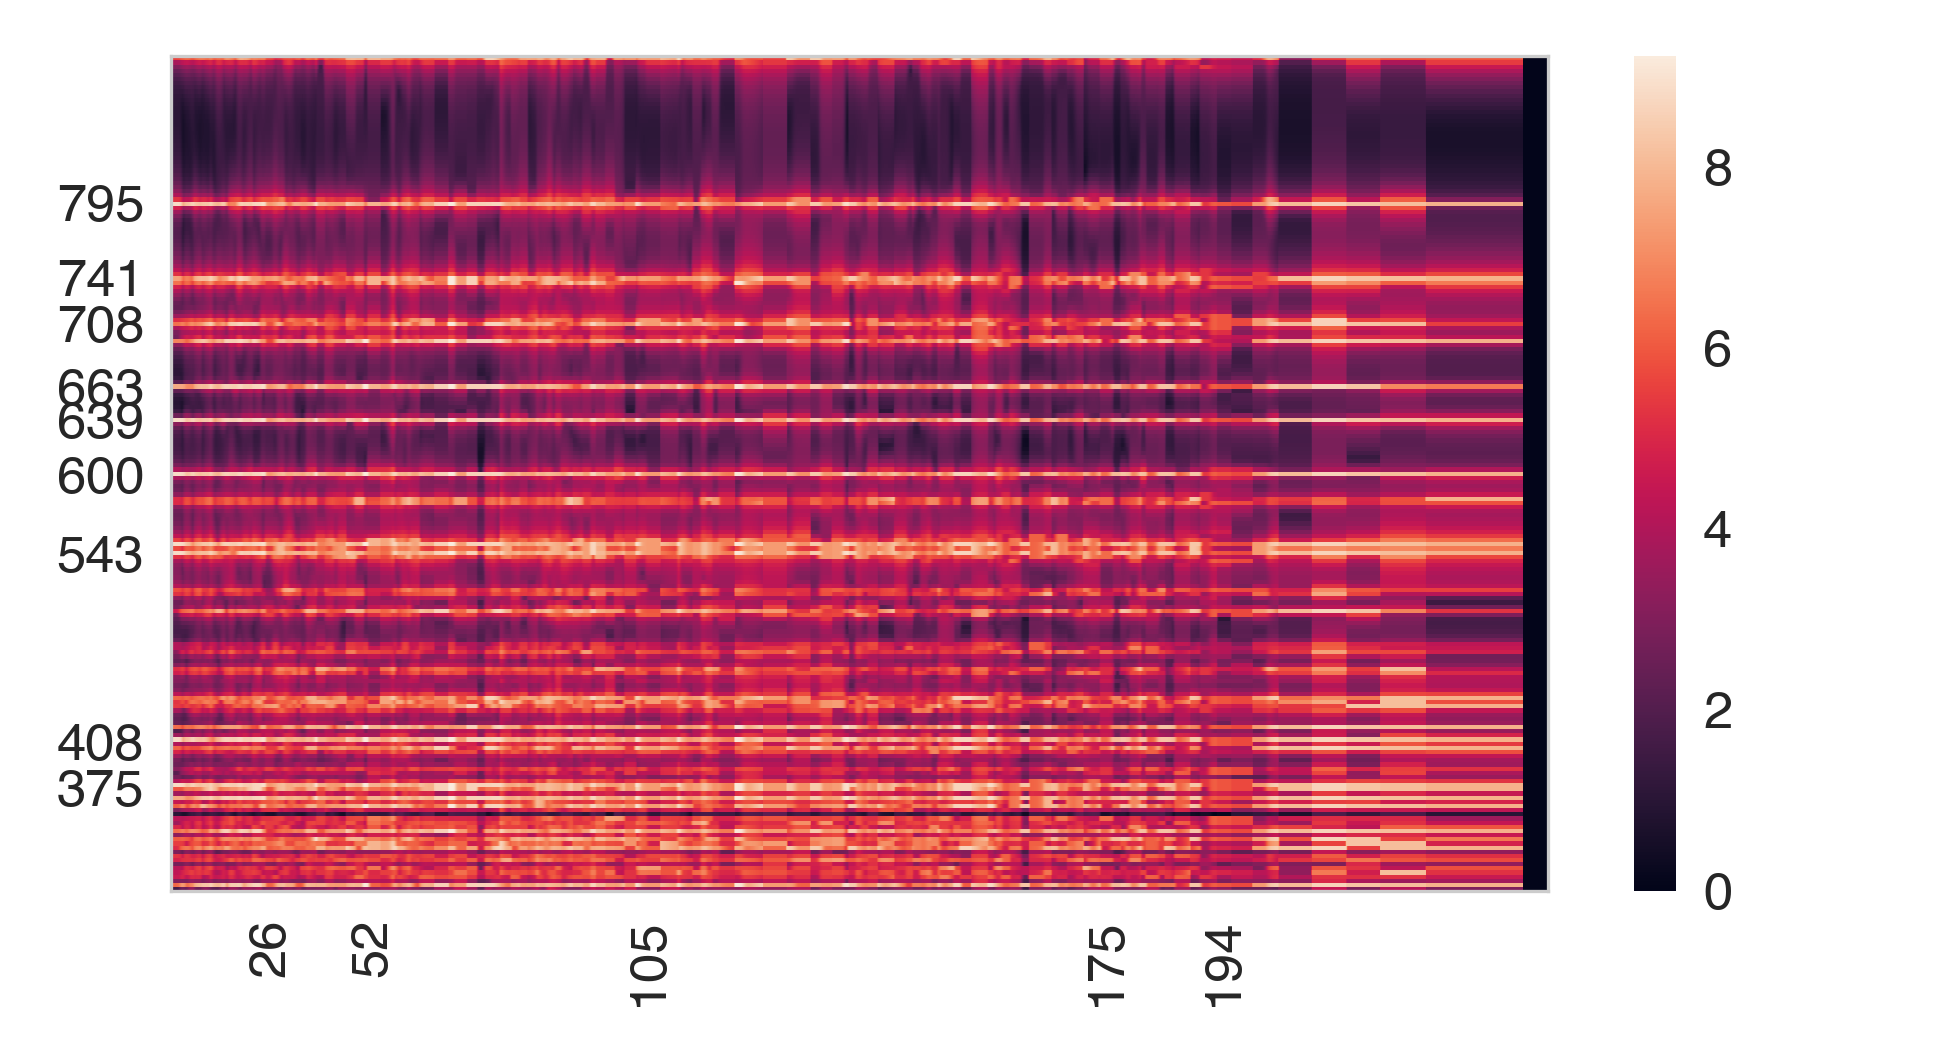
\includegraphics{comb-as12}\caption{Combined graph for As12-STX}\end{subfigure}
\begin{subfigure}{8.25cm}\centering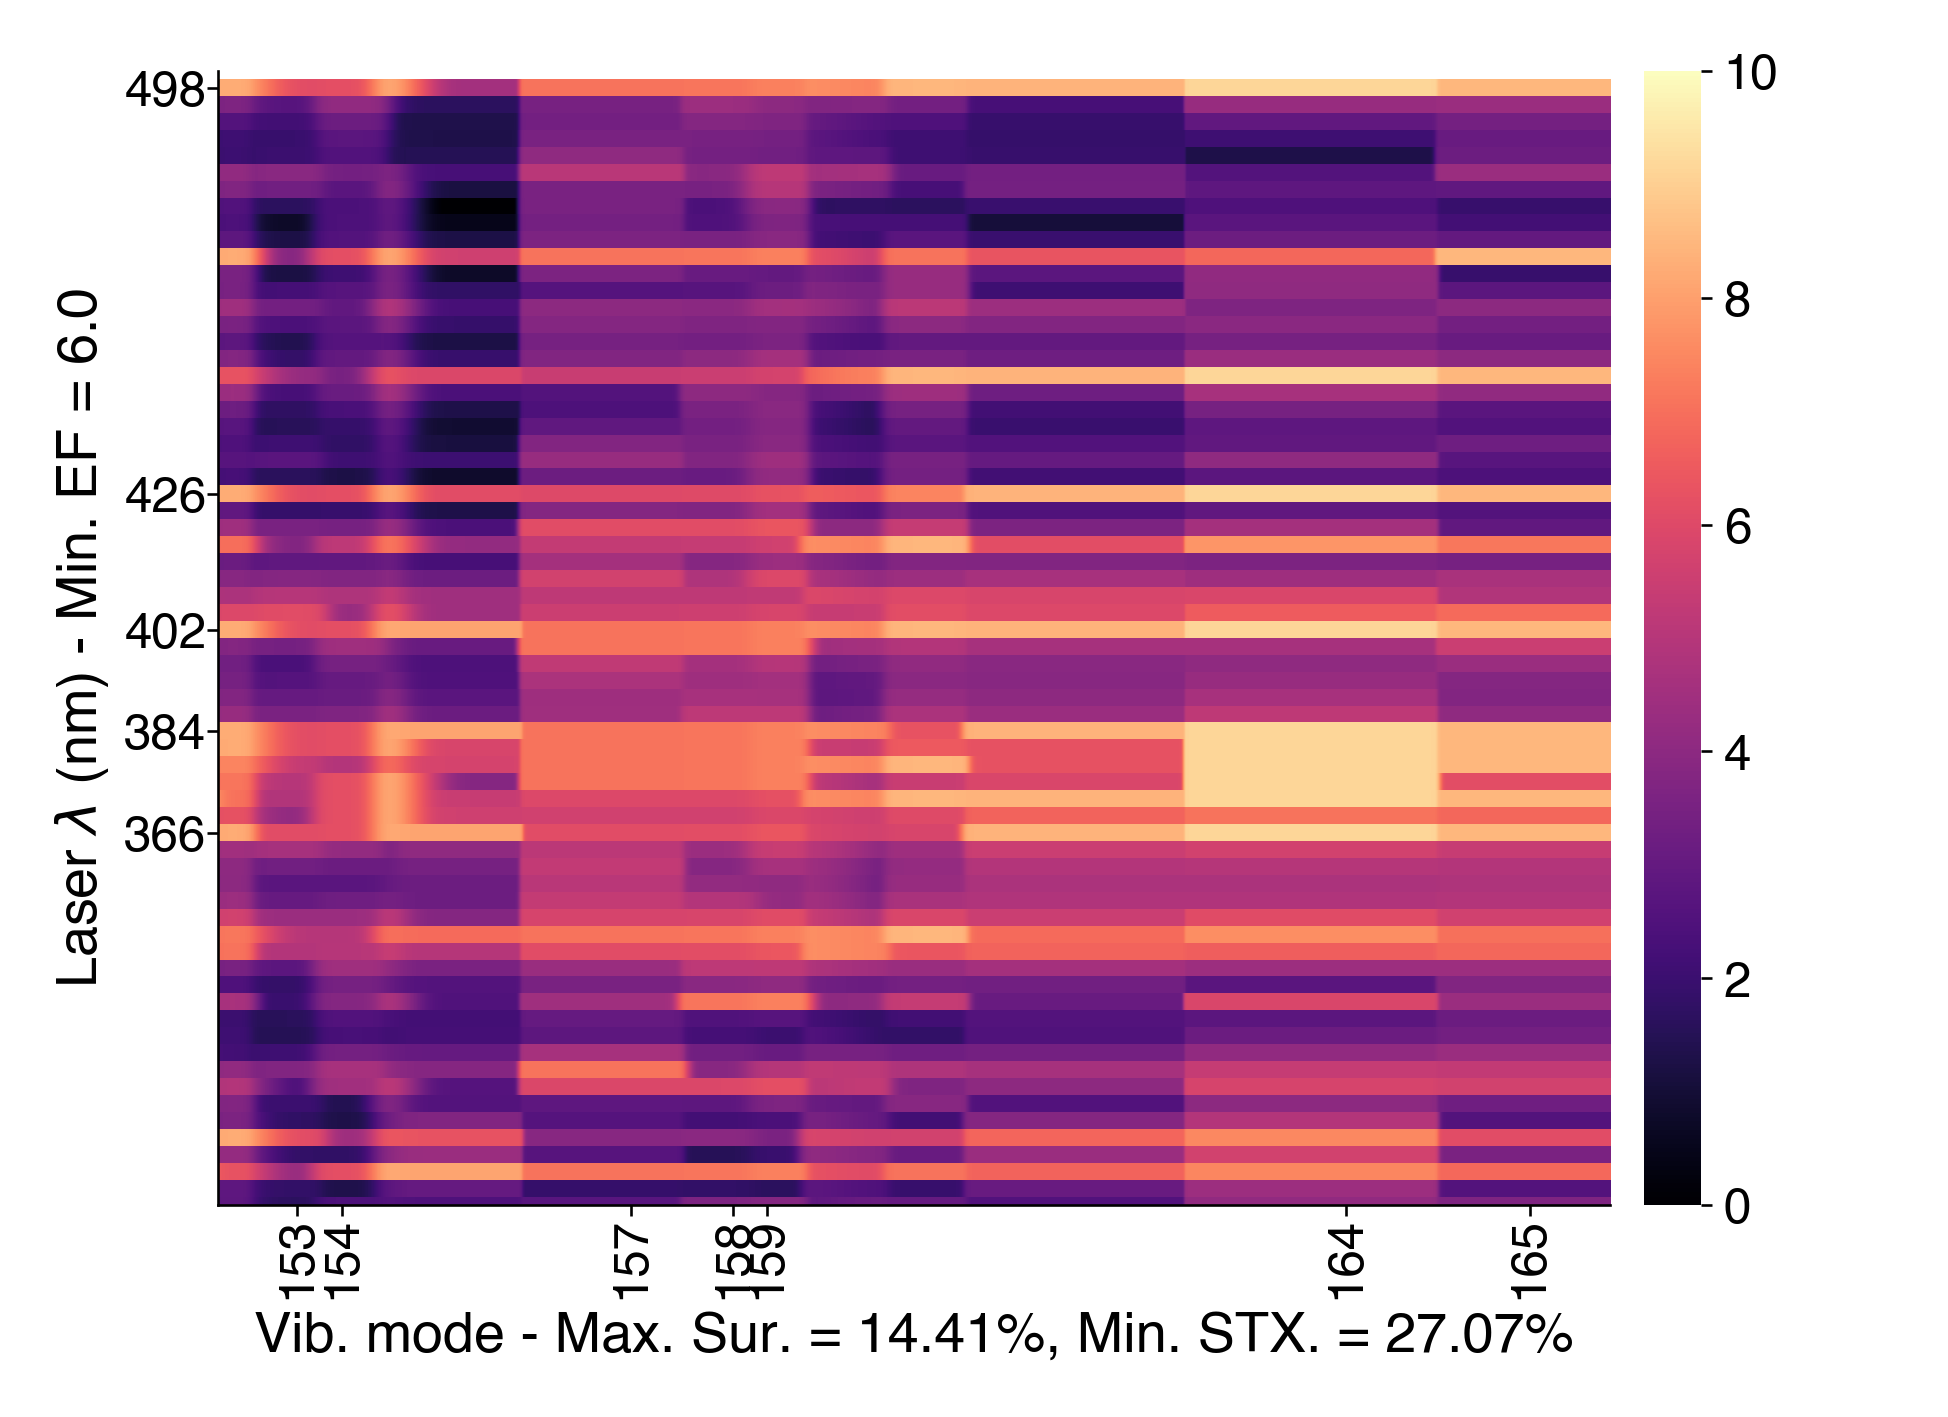
\includegraphics{comb-asn08}\caption{Combined graph for AsN08-STX}\end{subfigure}%
\begin{subfigure}{8.25cm}\centering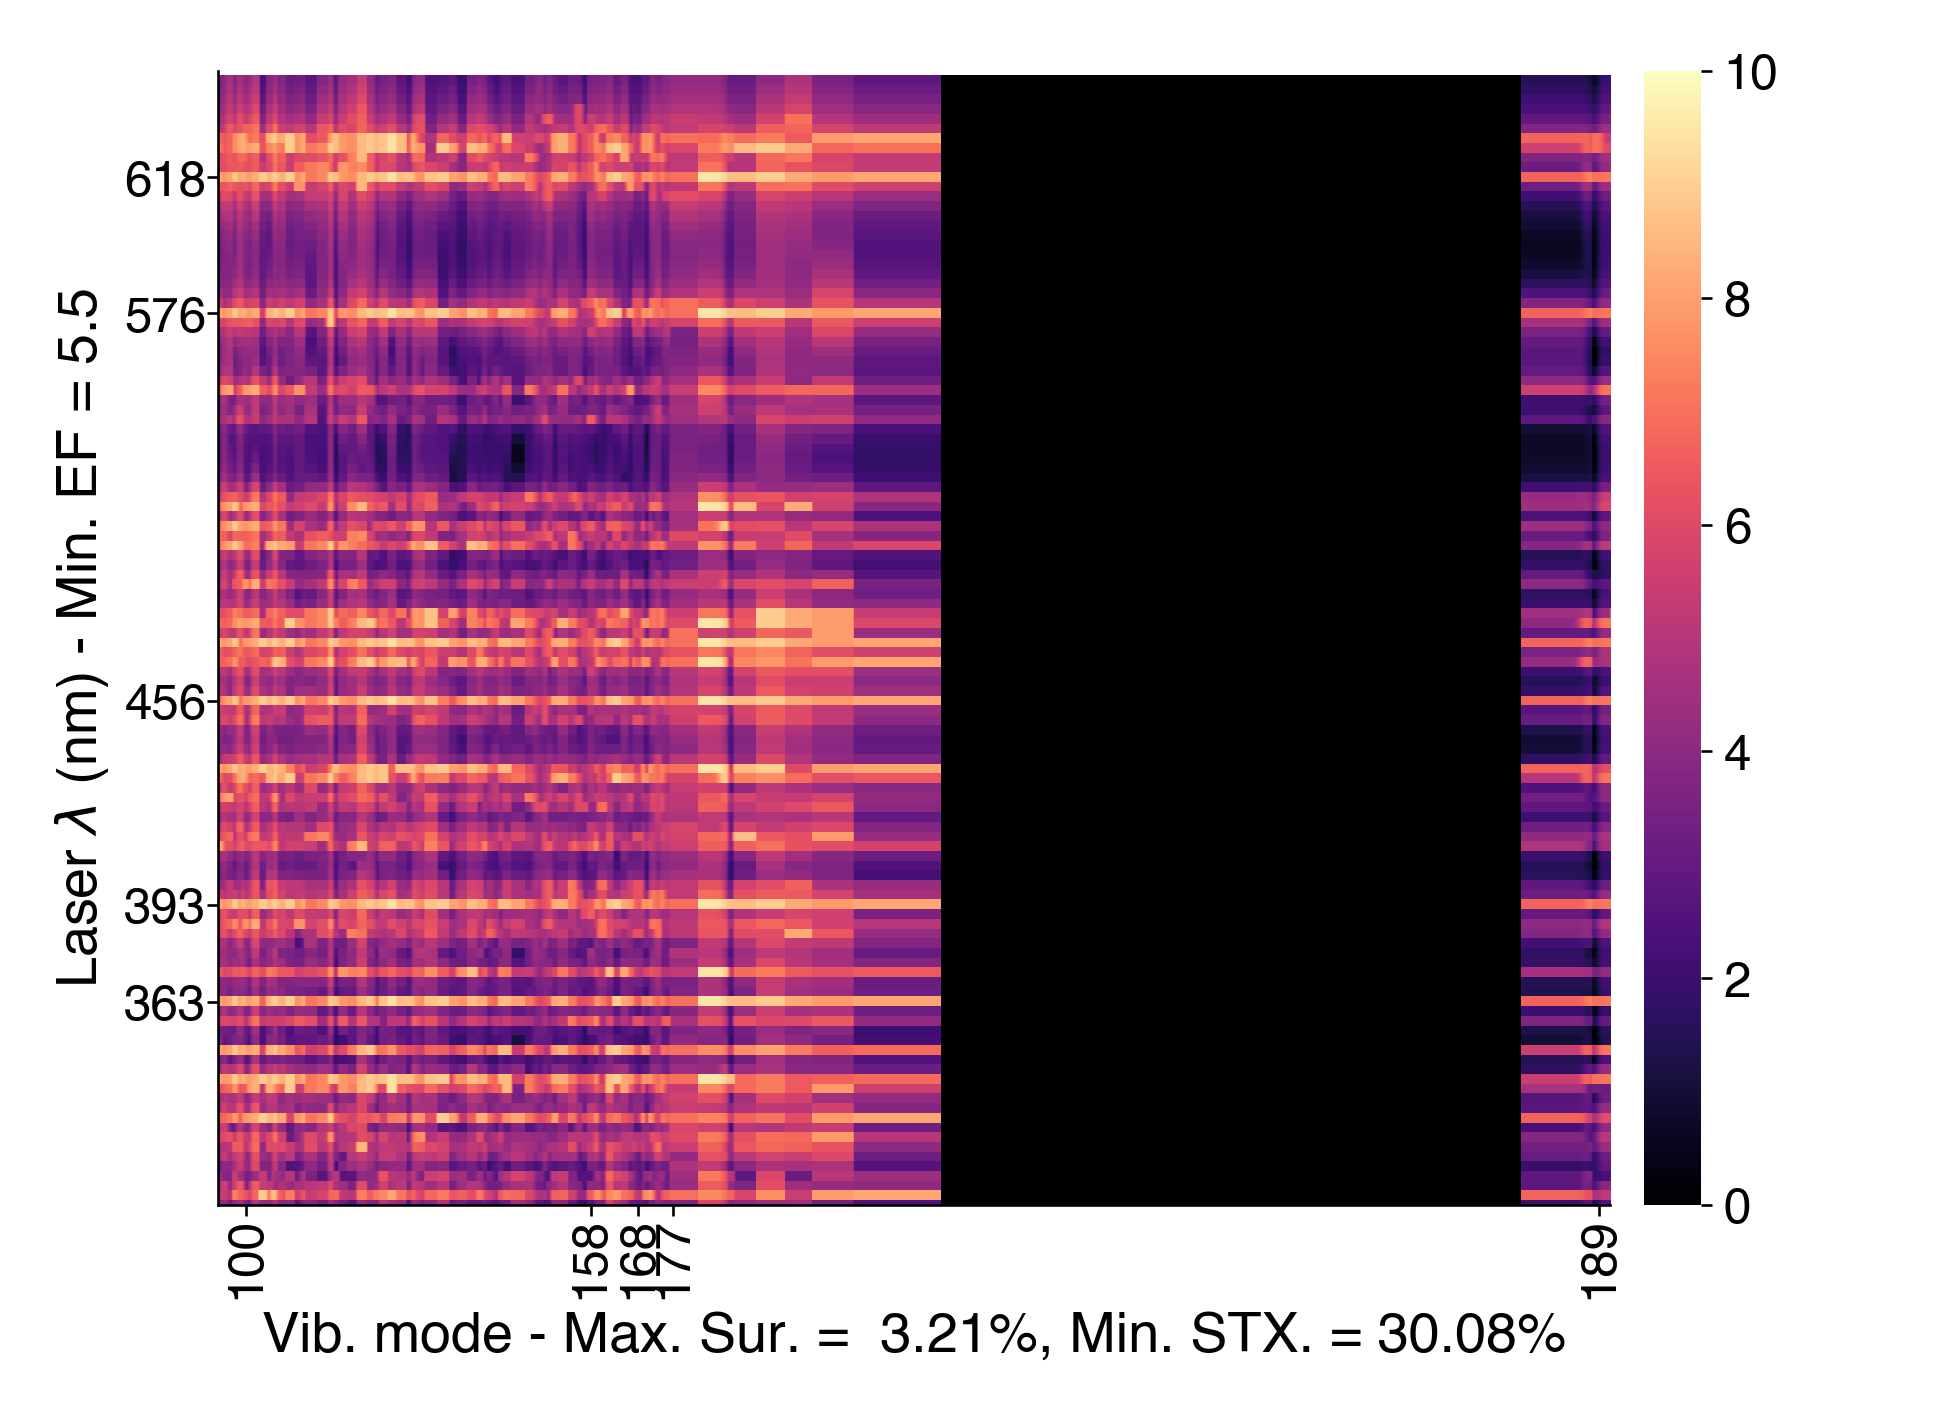
\includegraphics{comb-asn10}\caption{Combined graph for AsN10-STX}\end{subfigure}
\caption[Part 1 of combined EF RR graphs]{Part 1 of combined EF RR graphs}
\end{figure*}

\newpage

\begin{figure*}[h]
\centering
\begin{subfigure}{8.25cm}\centering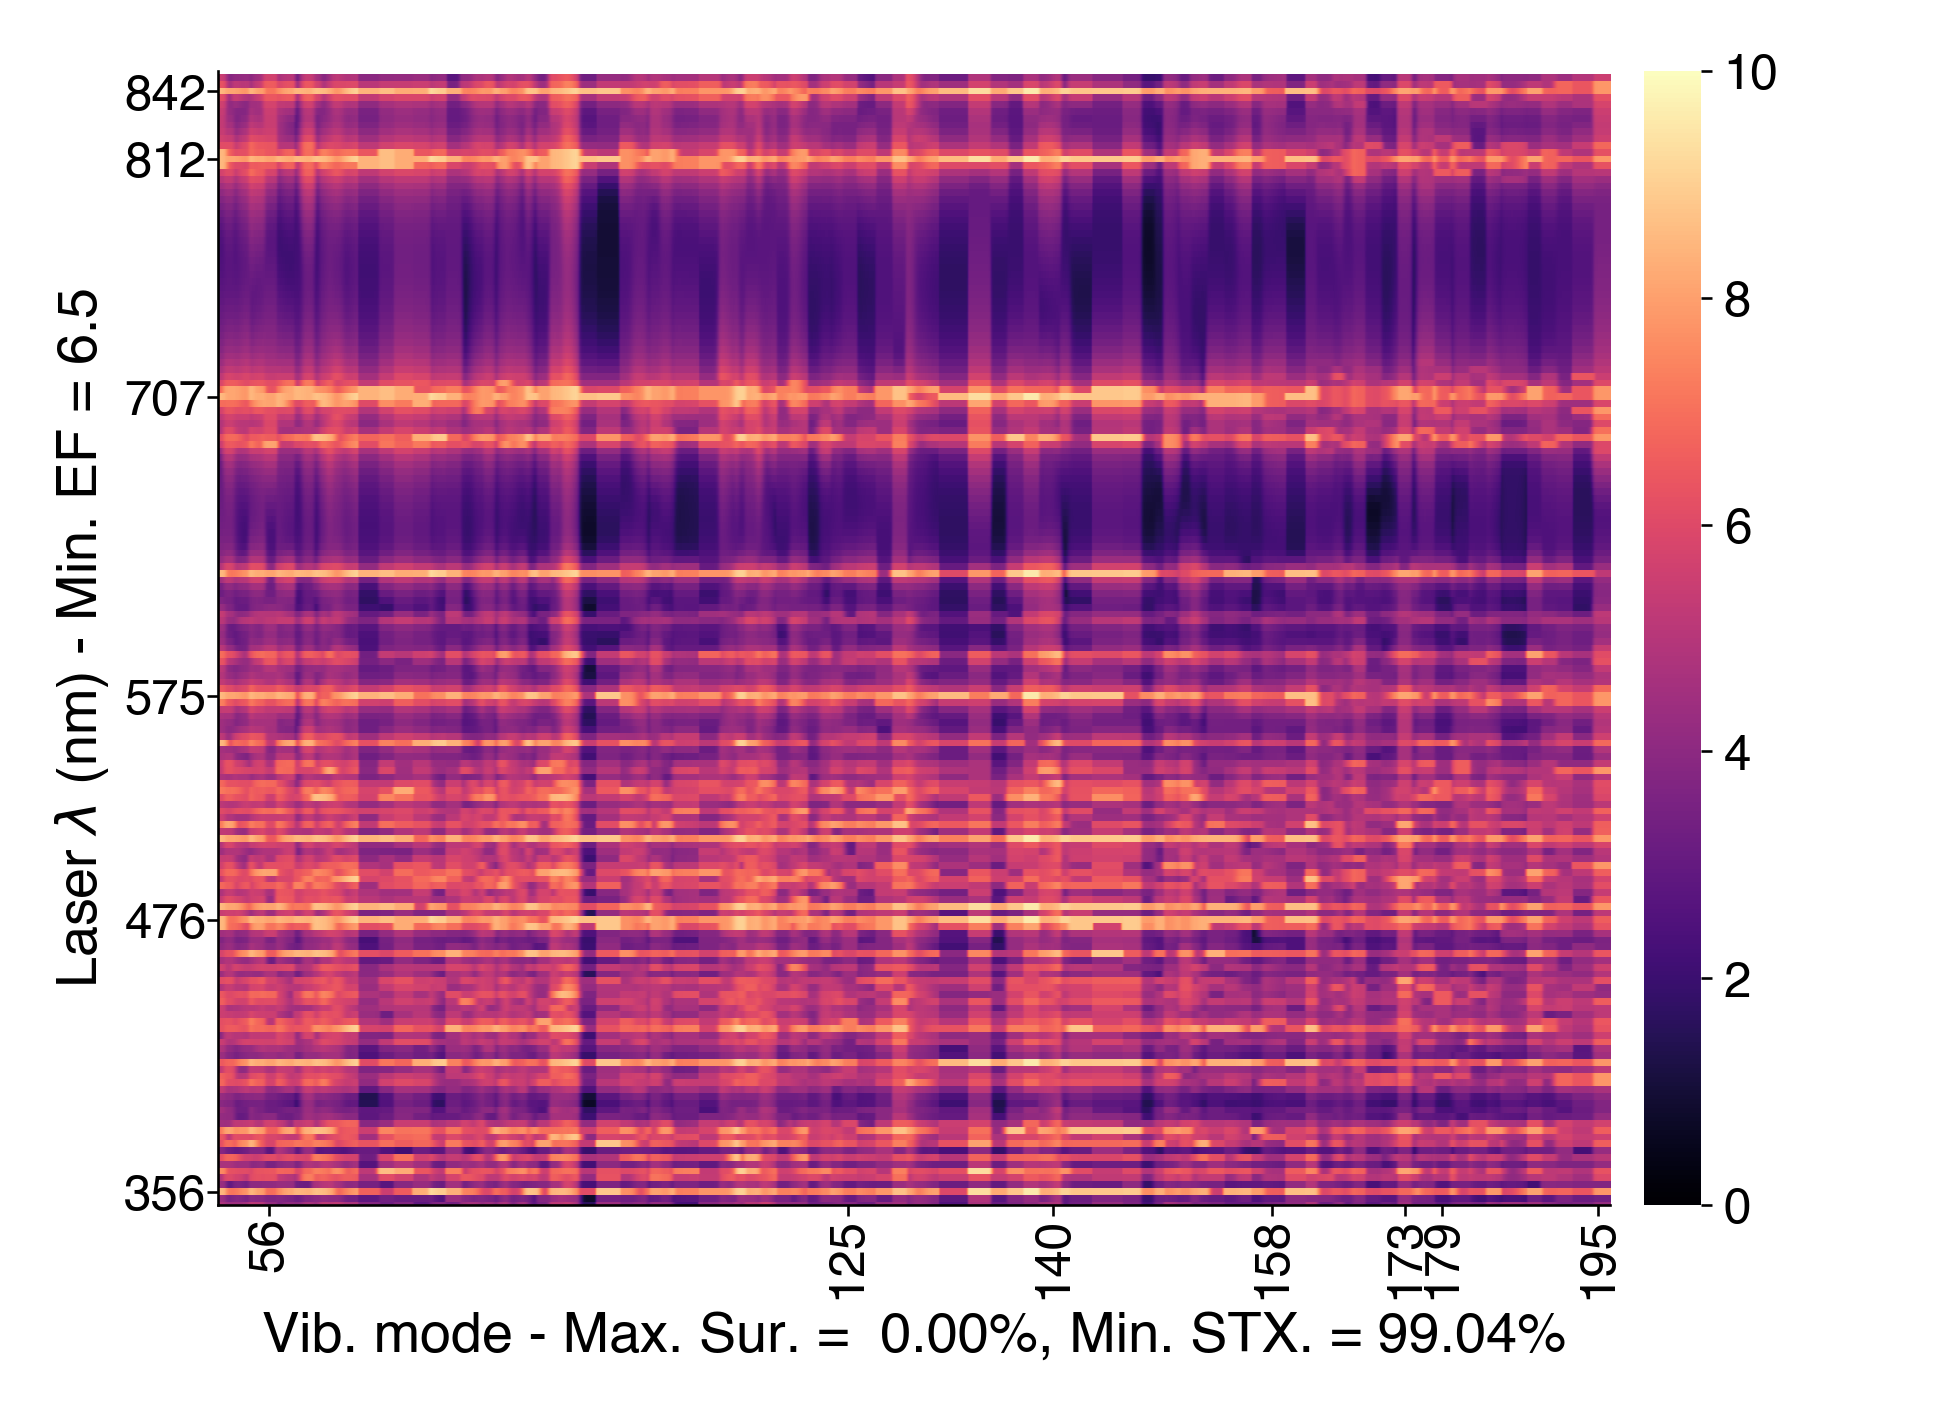
\includegraphics{comb-asn12}\caption{Combined graph for AsN12-STX}\end{subfigure}%
\begin{subfigure}{8.25cm}\centering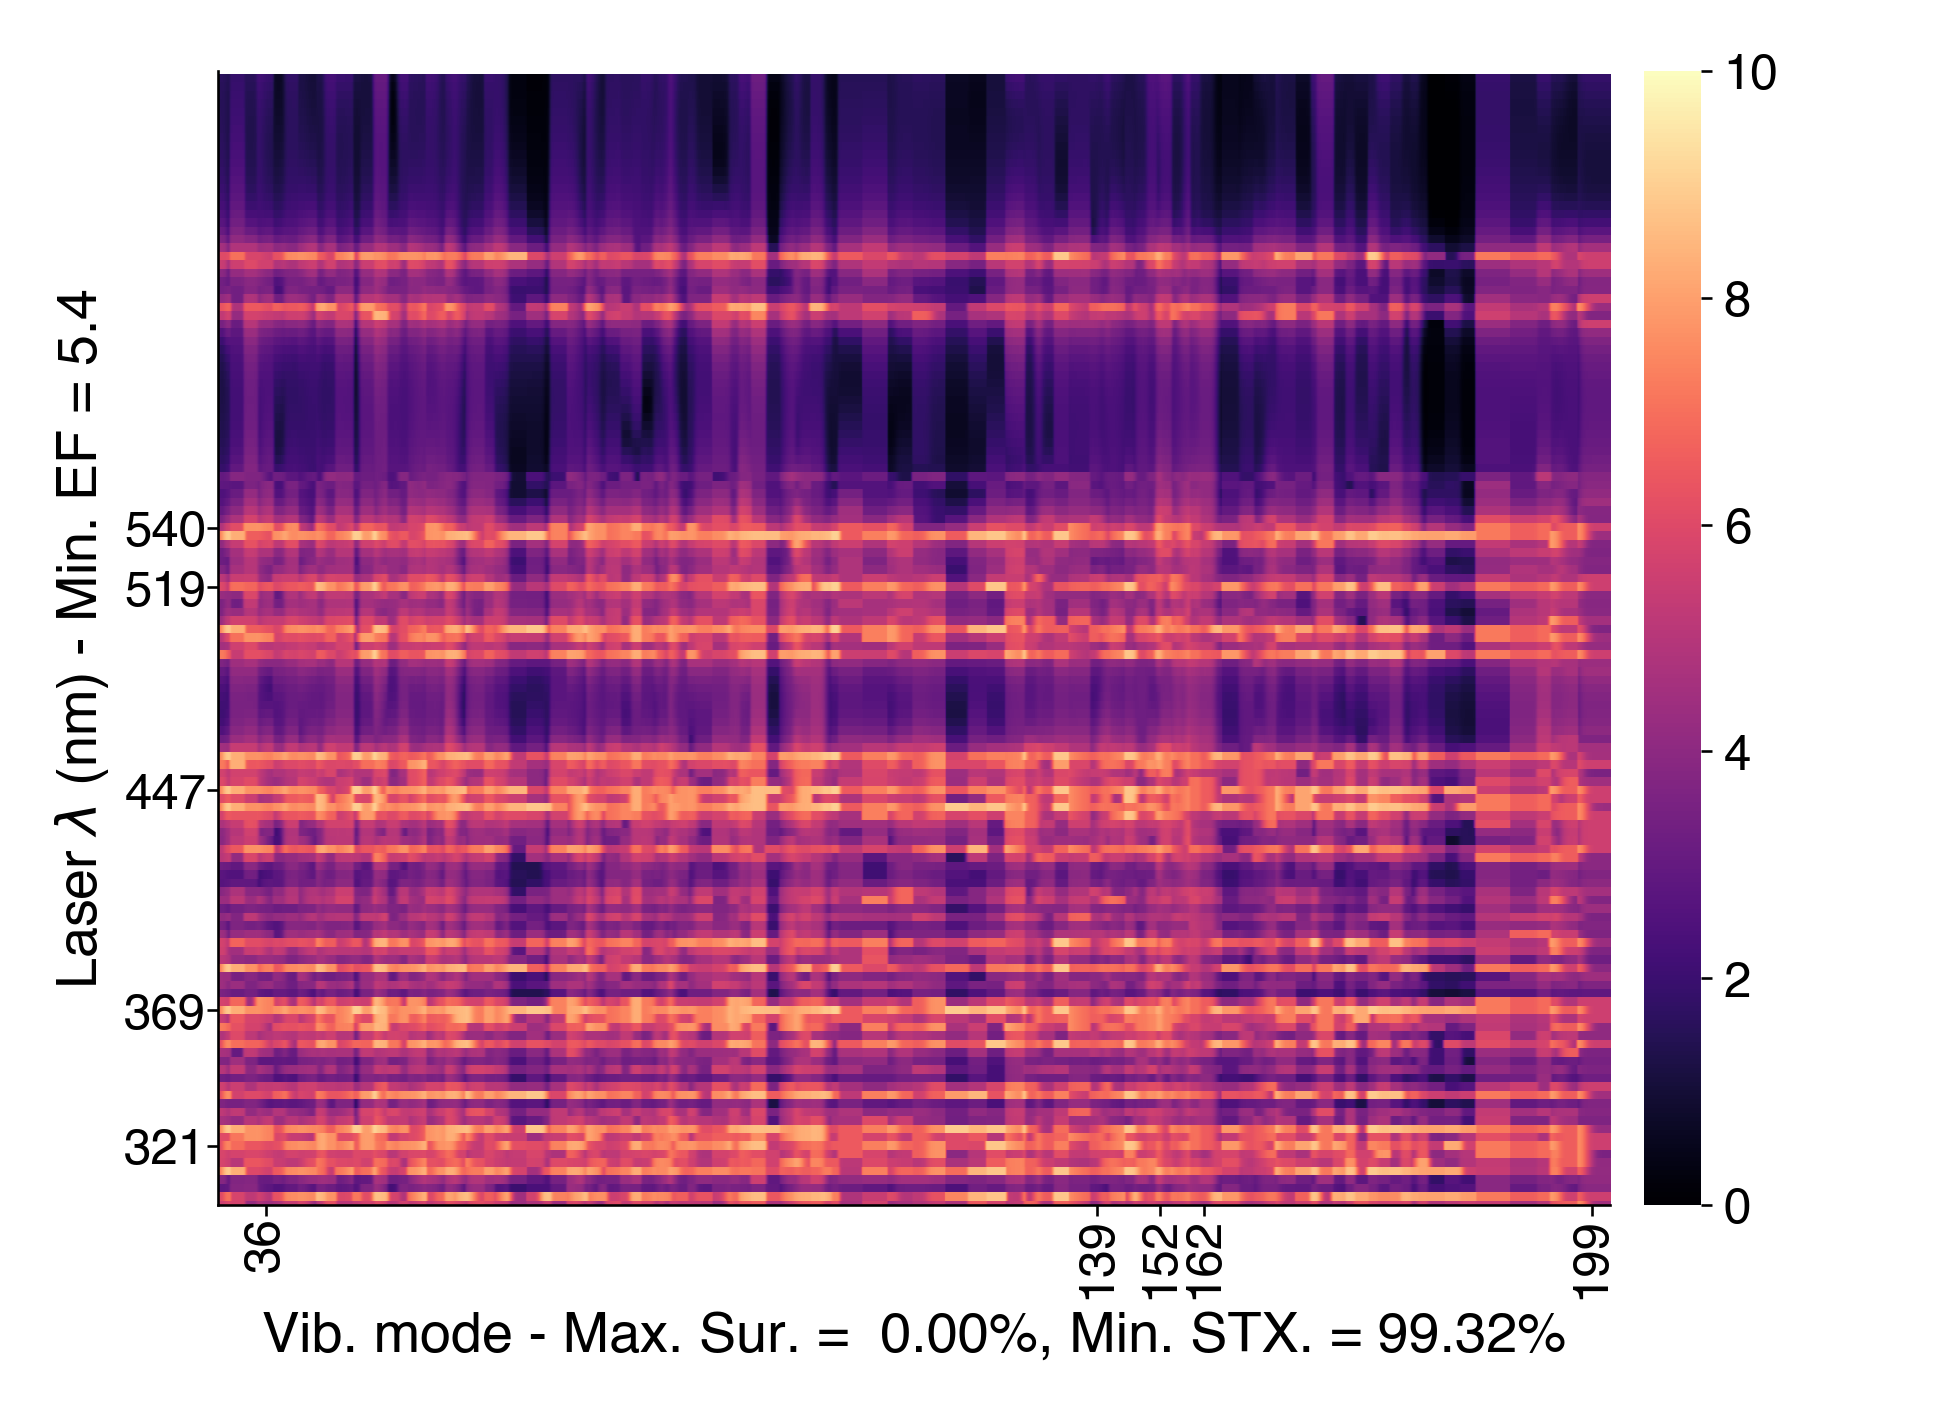
\includegraphics{comb-p12}\caption{Combined graph for P12-STX}\end{subfigure}
\begin{subfigure}{8.25cm}\centering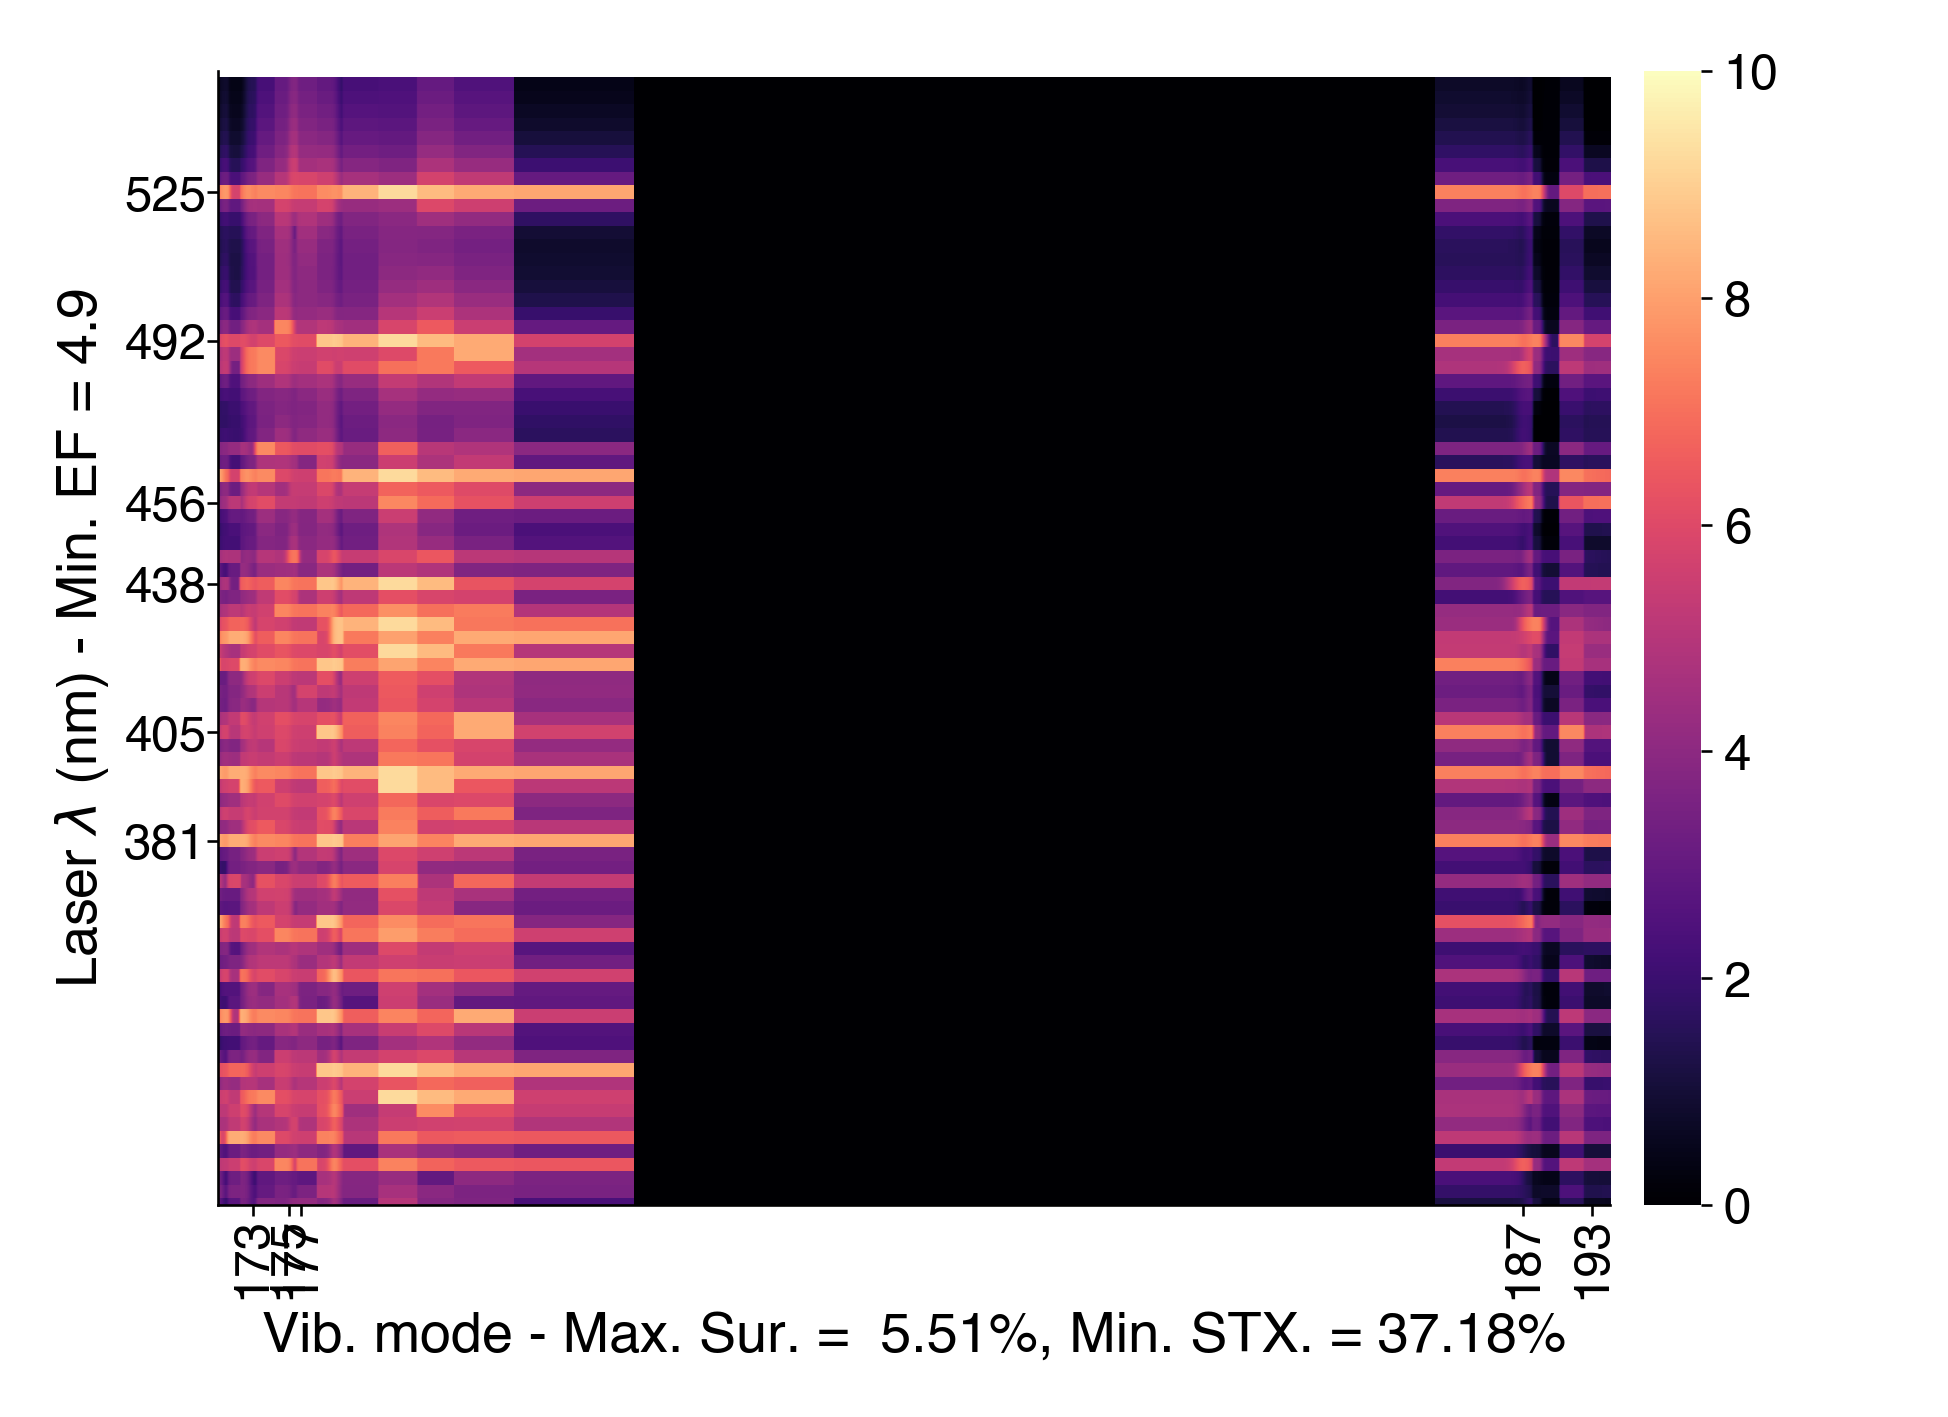
\includegraphics{comb-pn10}\caption{Combined graph for PN10-STX}\end{subfigure}%
\begin{subfigure}{8.25cm}\centering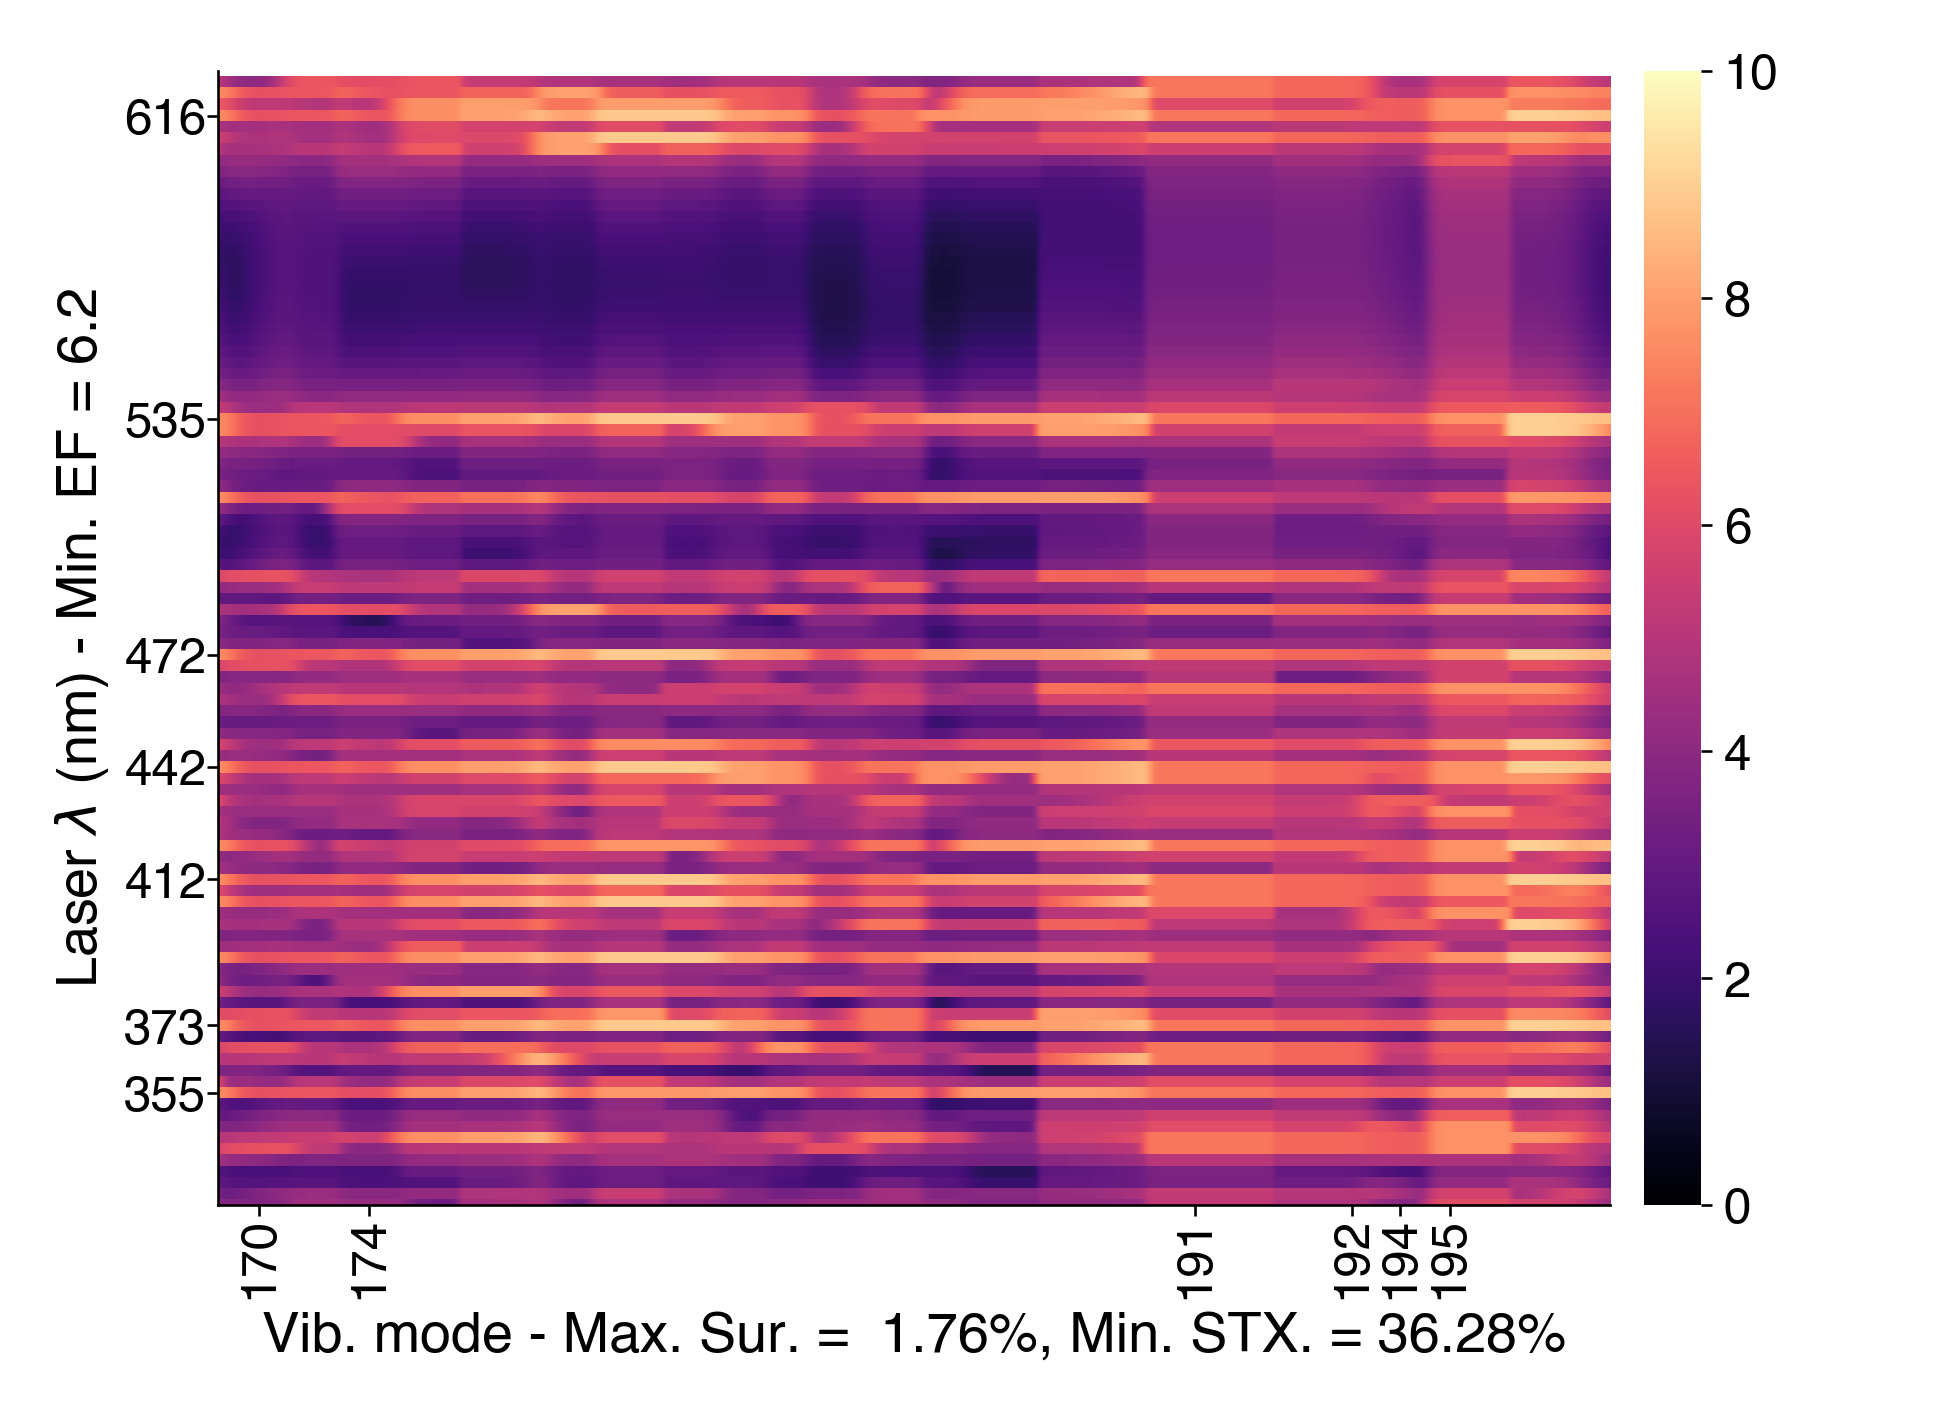
\includegraphics{comb-pn12}\caption{Combined graph for PN12-STX}\end{subfigure}
\caption[Part 2 of combined EF RR graphs]{Part 2 of combined EF RR graphs}
\end{figure*}


\newpage
\section{Resonance Raman spectra}
\labsec{ap:rr}

\begin{figure*}[h]
    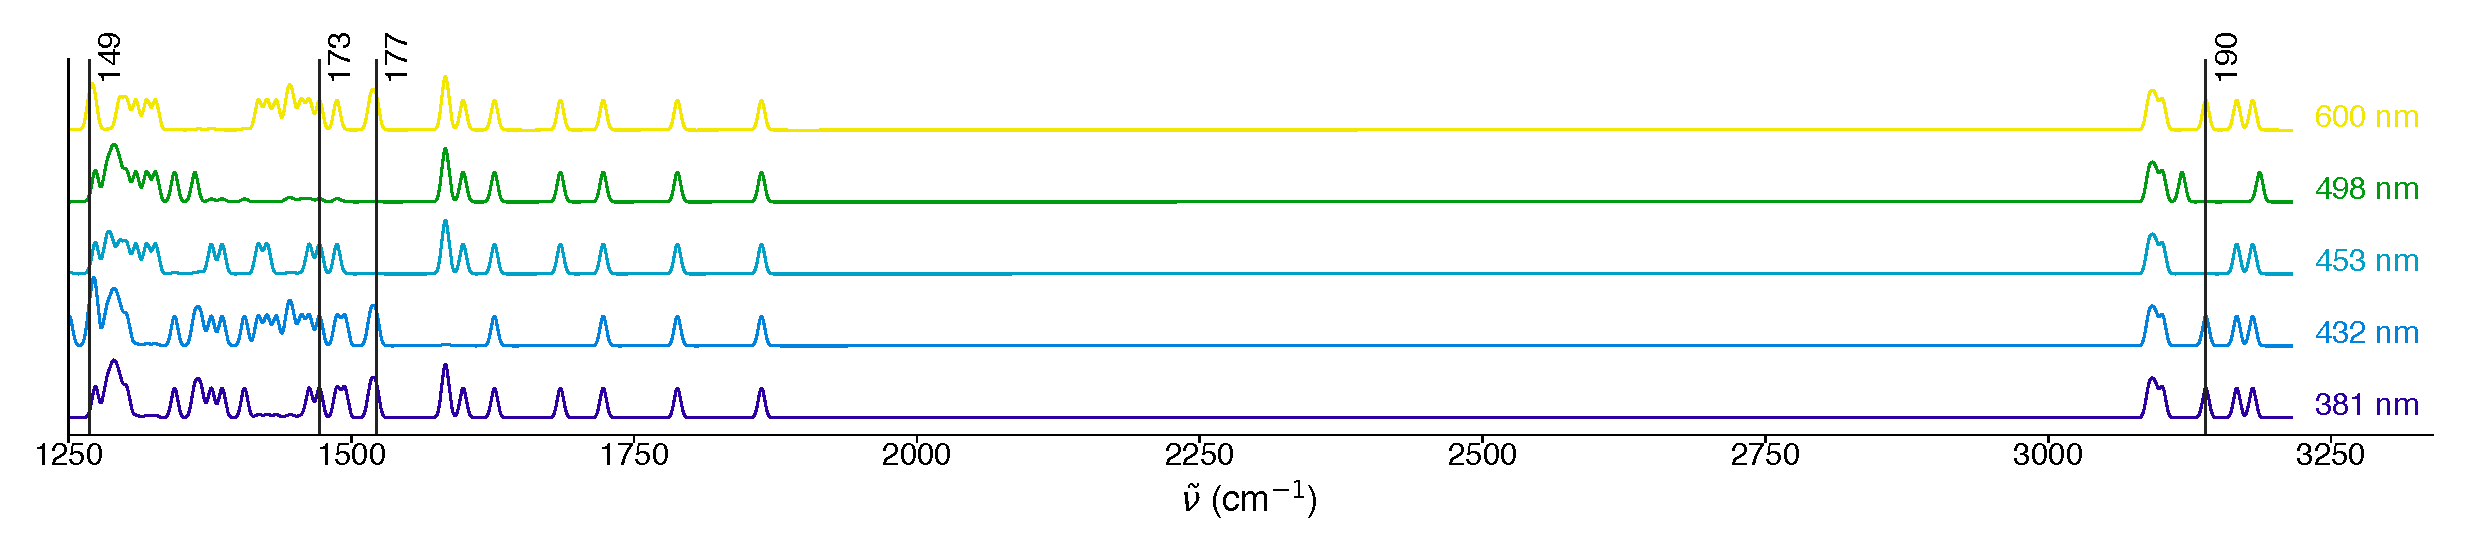
\includegraphics{unfolded-as10}
    \caption[RR spectra of As10-STX]{RR spectra of As10-STX. Selected $\lambda$: \SI{381}{\nano\metre}, \SI{432}{\nano\metre}, \SI{600}{\nano\metre}}
    \labfig{unfolded-as10}
\end{figure*}
\begin{figure*}[h]
    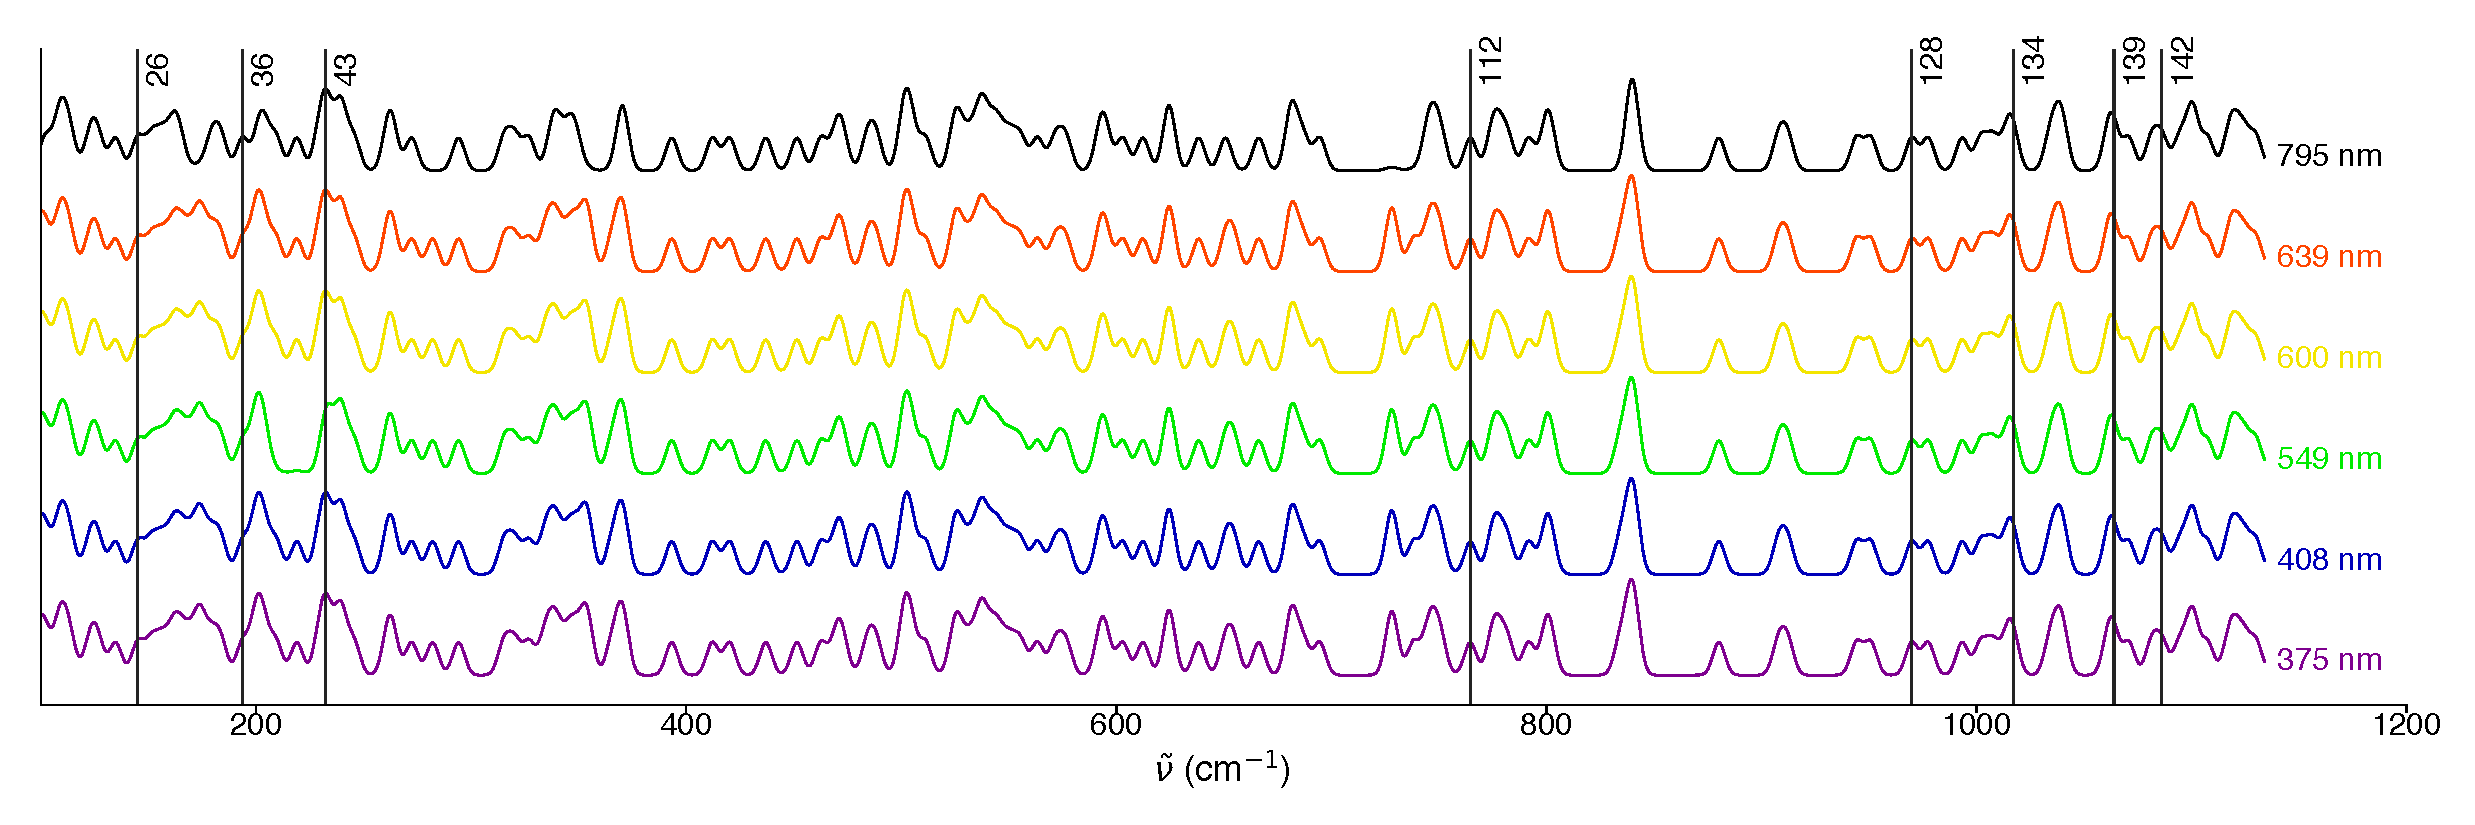
\includegraphics{unfolded-as12}
    \caption[RR spectra of As12-STX]{RR spectra of As12-STX. All of the lasers performed very similarly}
    \labfig{unfolded-as12}
\end{figure*}
\begin{figure*}[h]
    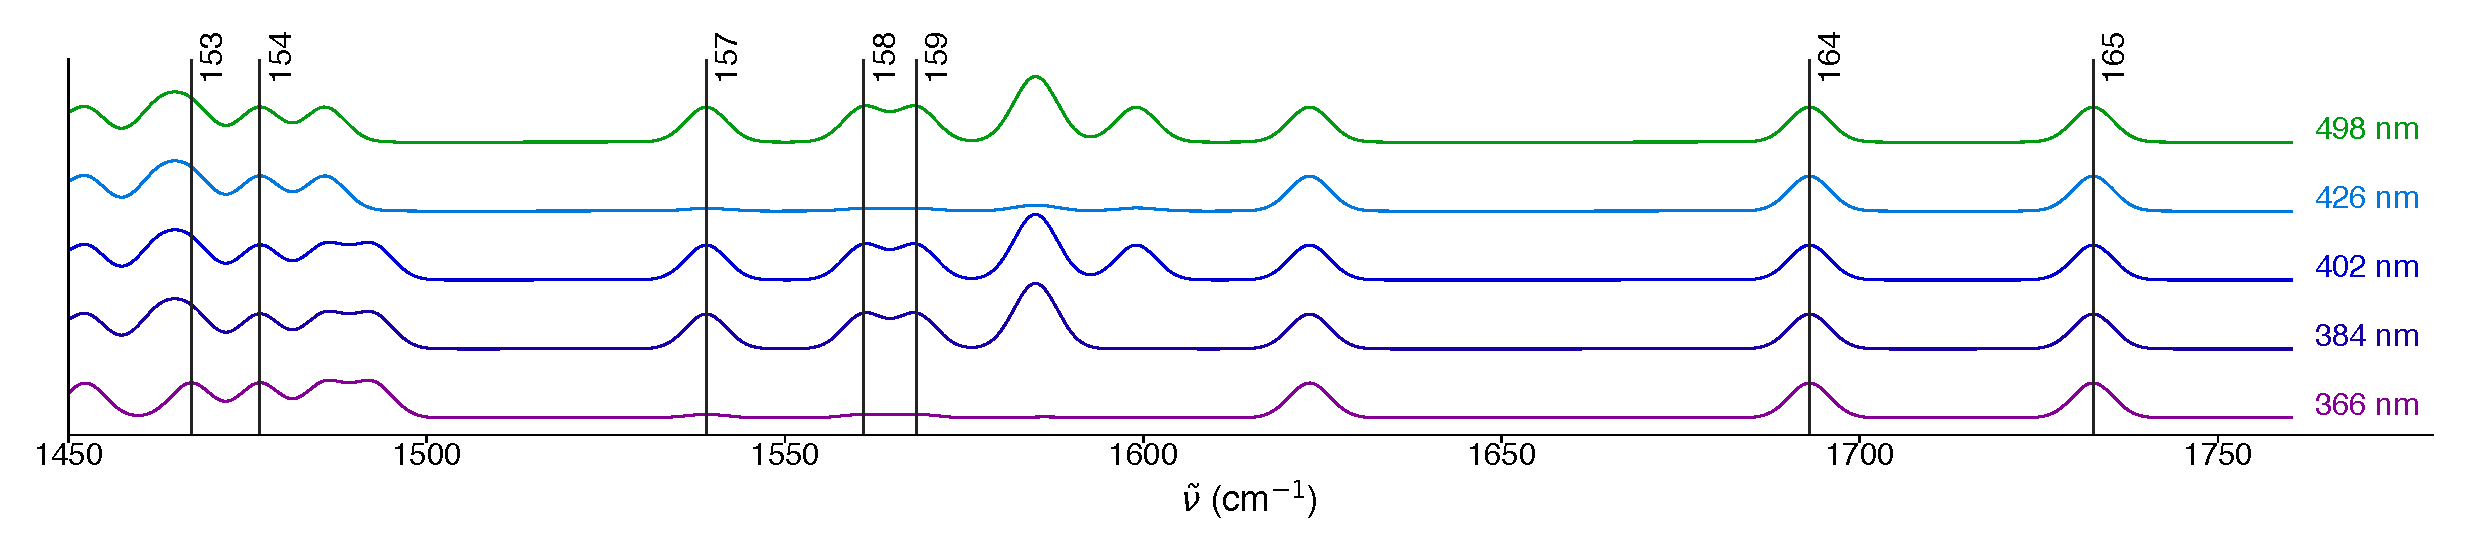
\includegraphics{unfolded-asn08}
    \caption[RR spectra of AsN08-STX]{RR spectra of AsN08-STX. Selected $\lambda$: \SI{384}{\nano\metre}, \SI{402}{\nano\metre}, \SI{498}{\nano\metre}}
    \labfig{unfolded-asn08}
\end{figure*}
\begin{figure*}[h]
    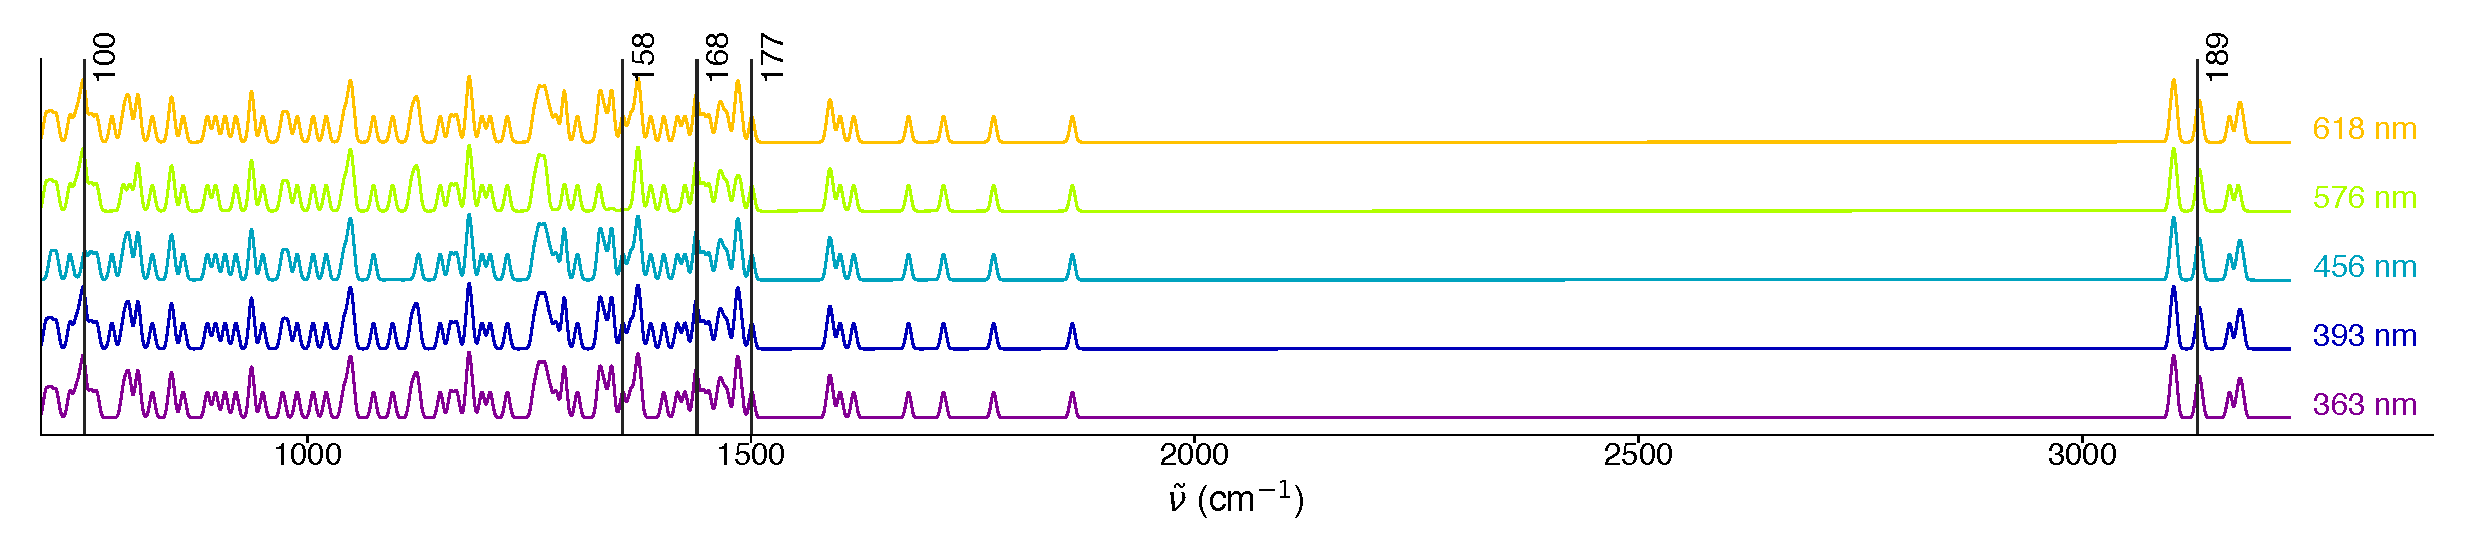
\includegraphics{unfolded-asn10}
    \caption[RR spectra of AsN10-STX]{RR spectra of AsN10-STX. All of the tested lasers resulted in similar amplifications}
    \labfig{unfolded-asn10}
\end{figure*}

\newpage

\begin{figure*}[h]
    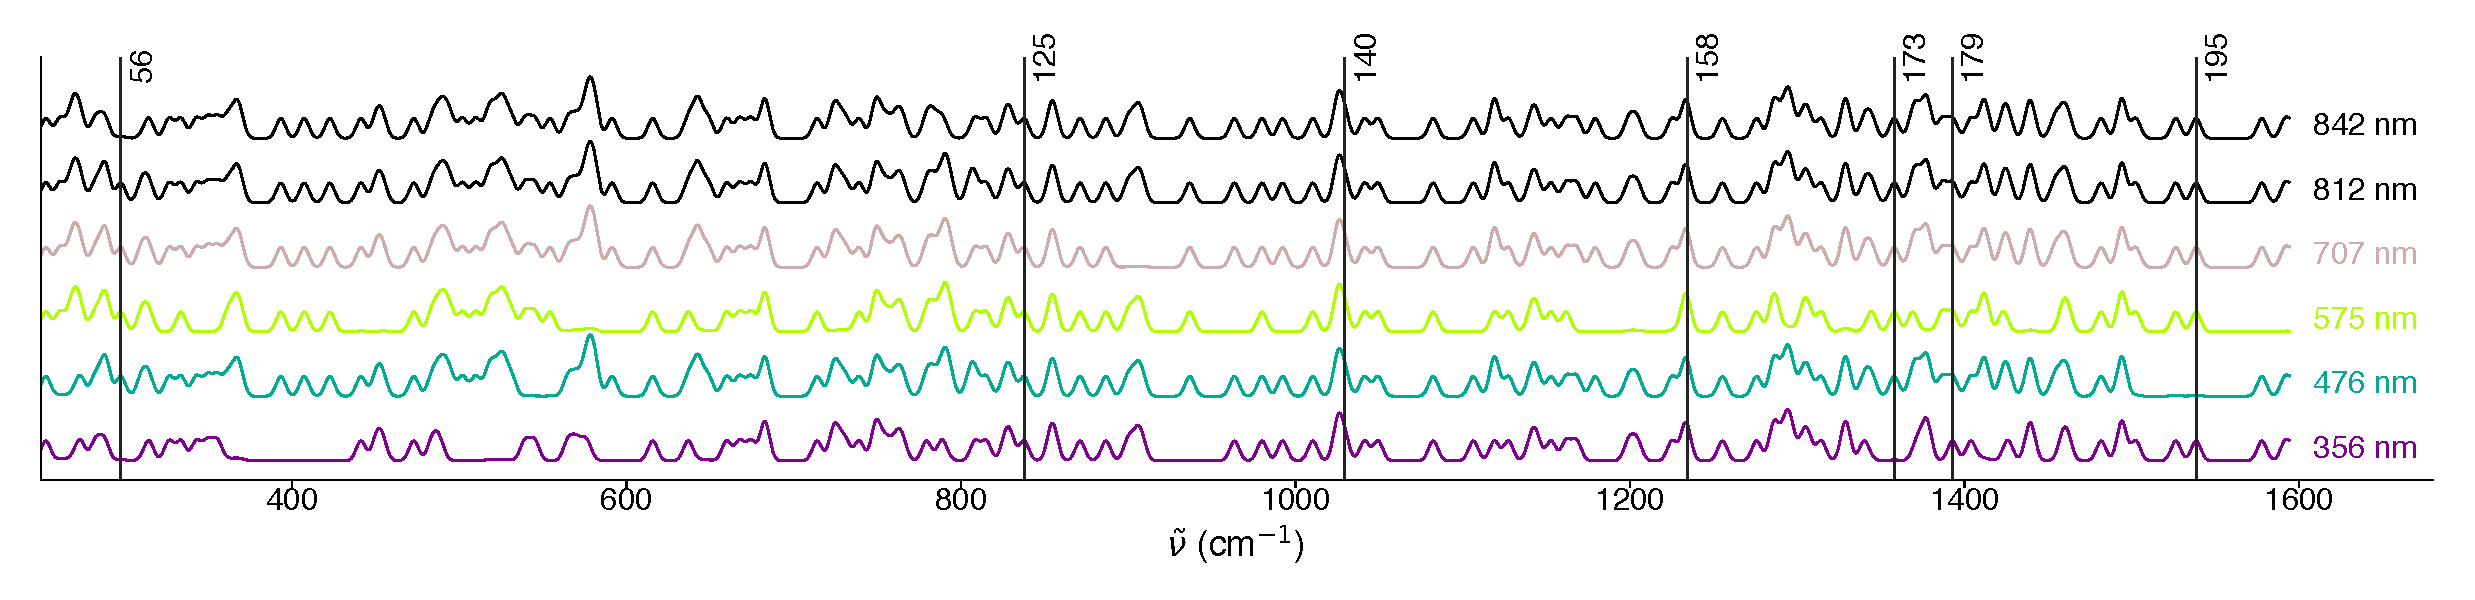
\includegraphics{unfolded-asn12}
    \caption[RR spectra of AsN12-STX]{RR spectra of AsN12-STX. All of the lasers were considered equivalent in terms of amplifications, except for \SI{476}{\nano\metre}, which did not amplify mode 195}
    \labfig{unfolded-asn12}
\end{figure*}
\begin{figure*}[h]
    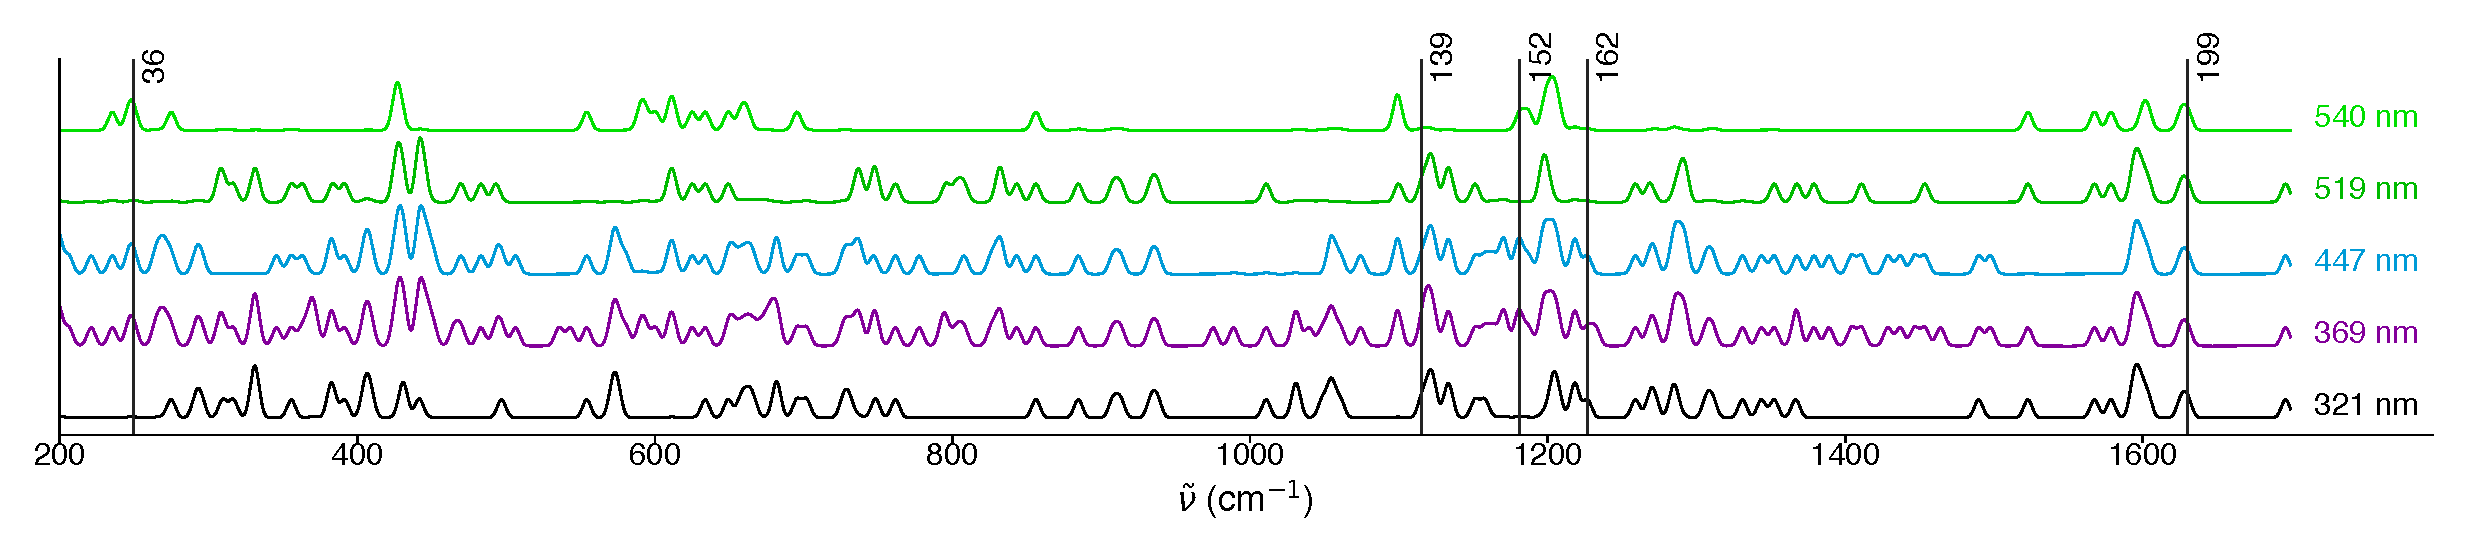
\includegraphics{unfolded-p12}
    \caption[RR spectra of P12-STX]{RR spectra of P12-STX. Selected $\lambda$: \SI{369}{\nano\metre}, \SI{447}{\nano\metre}}
    \labfig{unfolded-p12}
\end{figure*}
\begin{figure*}[h]
    \includegraphics{unfolded-pn10}
    \caption[RR spectra of PN10-STX]{RR spectra of PN10-STX. Selected $\lambda$: \SI{381}{\nano\metre}, \SI{525}{\nano\metre}}
    \labfig{unfolded-pn10}
\end{figure*}
\begin{figure*}[h]
    \includegraphics{unfolded-pn12}
    \caption[RR spectra of PN12-STX]{RR spectra of PN12-STX. All of the wavelengths were considered suitable}
    \labfig{unfolded-pn12}
\end{figure*}


\newpage
\section{Best Resonance Raman and derivatives}
\labsec{ap:rr-diff}

\begin{figure*}[h]
    \includegraphics{final-as10}
    \caption[RR spectra of As10-STX at \SI{381}{\nano\metre}]{RR spectra of As10-STX at \SI{381}{\nano\metre}}
    \labfig{final-as10}
\end{figure*}
\begin{figure*}[h]
    \includegraphics{final-as12}
    \caption[RR spectra of As12-STX at \SI{543}{\nano\metre}]{RR spectra of As12-STX at \SI{543}{\nano\metre}}
    \labfig{final-as12}
\end{figure*}
\begin{figure*}[h]
    \includegraphics{final-asn08}
    \caption[RR spectra of AsN08-STX at \SI{498}{\nano\metre}]{RR spectra of AsN08-STX at \SI{498}{\nano\metre}}
    \labfig{final-asn08}
\end{figure*}
\begin{figure*}[h]
    \includegraphics{final-asn10}
    \caption[RR spectra of AsN10-STX at \SI{618}{\nano\metre}]{RR spectra of AsN10-STX at \SI{618}{\nano\metre}}
    \labfig{final-asn10}
\end{figure*}

\newpage

\begin{figure*}[h]
    \includegraphics{final-asn12}
    \caption[RR spectra of AsN12-STX at \SI{707}{\nano\metre}]{RR spectra of AsN12-STX at \SI{707}{\nano\metre}}
    \labfig{final-asn12}
\end{figure*}
\begin{figure*}[h]
    \includegraphics{final-p12}
    \caption[RR spectra of P12-STX at \SI{447}{\nano\metre}]{RR spectra of P12-STX at \SI{447}{\nano\metre}}
    \labfig{final-p12}
\end{figure*}
\begin{figure*}[h]
    \includegraphics{final-pn10}
    \caption[RR spectra of PN10-STX at \SI{525}{\nano\metre}]{RR spectra of PN10-STX at \SI{525}{\nano\metre}}
    \labfig{final-pn10}
\end{figure*}
\begin{figure*}[h]
    \includegraphics{final-pn12}
    \caption[RR spectra of PN12-STX at \SI{616}{\nano\metre}]{RR spectra of PN12-STX at \SI{616}{\nano\metre}}
    \labfig{final-pn12}
\end{figure*}
